
\chapter{Structure de séquences réparties à large échelle}
\minitoc

\TODO{Work on an introduction.}


\section{État de l'art}
\label{repl:sec:replication}

La maintenance de répliques sur des machines distantes les unes des
autres est un problème ancien. Dès 1975, les bases de données répliquées font
leur apparition~\cite{johnson1975maintenance} afin de résoudre
\begin{inparaenum}[(i)]
\item les problèmes de défaillances~\cite{alsberg1976principle}, i.e., le
  serveur possédant les données étant inaccessible, le client peut contacter
  serveur alternatif connu pour posséder les mêmes données afin de satisfaire sa
  requête;
\item les problèmes de rapidité d'accès, i.e., le client peut contacter un
  serveur dont la latence est la plus faible afin de satisfaire plus rapidement
  sa requête.
\end{inparaenum}

Hélas, avec la réplication, la synchronisation de répliques devient le coeur du
problème. Puisque la communication entre serveurs n'est pas instantanée, les
modifications effectuées sur les données prennent du temps à parvenir aux
répliques. Cela implique des problèmes de
\begin{inparaenum}[(i)]
\item fraîcheur de données -- \emph{est-ce que la donnée que j'obtiens est la
    plus à jour?} -- et de
\item modifications concurrentes -- \emph{avec des modifications effectuées sur
    une même données, au même moment, par deux serveurs distants dont les
    résultats sont différents. Dois-je conserver les deux modifications, ou
    dois-je en privilégier une, ou dois-je employer une autre stratégie?}
\end{inparaenum}


Hélas, d'après le théorème CAP~\cite{gilbert2002brewer} il est impossible de
répliquer sur un grand nombre de serveurs tout en garantissant à la fois :
\begin{itemize}
\item [\textbf{Cohérence :}] un contrat entre le développeur et la structure qui
  spécifie comment cette dernière se comporte suivant les opérations effectuées
  et leur ordonancement.
\item [\textbf{Disponibilité :}] le ratio entre le temps effectif durant lequel
  l'utilisateur accède à un service et le temps durant lequel il souhaite y
  accèder.
\item [\textbf{Tolérance aux pannes :}] les défaillances de serveurs
  n'entrainent pas une panne générale du système.
\end{itemize}

Face à ce constat, deux grandes familles de réplication : la réplication
pessimiste cherche à donner l'illusion d'une donnée unique lorsque la
réplication optimiste autorise à ses répliques de légères divergences
temporaires (cf. §\ref{repl:sec:schemas}). Cette dernière passant plus volontier
à l'échelle, nous nous intéresserons à deux familles d'approches y appartenant,
à savoir les transformés opérationnels dont les opérations sont modifiées à
l'intégration afin d'adapter l'opération au contexte d'exécution, et les
structures de données sans résolution de conflits dont les opérations commutent
(cf. §\ref{repl:sec:otorcrdts}). Finalement, la section~\ref{repl:sec:sequences}
s'intéresse plus particulièrement au type séquence, le plus proche d'un
document.

%%% Local Variables:
%%% mode: latex
%%% TeX-master: "../../paper"
%%% End:


\subsection{Pessimisme ou optimisme?}
\label{repl:subsec:schemas}

De multiples serveurs, possiblement distants les uns des autres, hébergent une
réplique d'une donnée. Lorsqu'une réplique est modifiée, sa modification est
répercutée sur les autres répliques. Les deux schémas de réplication définissent
la manière dont une modification est acceptée. Cela influe sur les propriétés du
système. En particulier, les dimensions que peuvent atteindre les systèmes, en
nombre de répliques, s'en trouve impactées.

\subsubsection{Réplication pessimiste}
\label{repl:subsubsec:pessimistic}

L'objectif de la réplication pessimiste est simple. Il consiste à donner
l'illusion que la donnée manipulée est unique, indépendemment du nombre de
répliques réel. Ainsi, il devient facile de raisonner sur les données puisque
leurs spécifications sont proches de celles proposées dans un contexte
non-réparti -- sans réplications.

Toutefois, avant qu'une modification ne soit réellement effectuée, il est
nécessaire qu'elles soient validées. L'autorité décisionnelle diffère en fonction
des approches :
\begin{itemize}
\item [\textbf{Autorité centrale~\cite{alsberg1976principle} :}] l'un des
  serveurs est désigné responsable. Ceux qui souhaitent modifier la donnée sont
  alors dans l'obligation de demander l'accès exclusif pendant la mise en place
  de cette modification. Dans l'intervalle, les autres répliques ne peuvent
  soumettre de modifications. Enfin, lorsque la modification est achevée, la
  main est rendue au serveur qui peut autoriser d'autres modifications. On parle
  de verrou (\emph{lock}).
\item [\textbf{Quorum~\cite{gifford1979weighted} :}] un ensemble de serveurs est
  désigné responsable. Chacune des modifications est soumise à un vote quant à
  son acceptation. Au dessus d'un certain seuil de vote positif ou négatif, la
  modification est autorisée ou non.
\end{itemize}


\begin{figure*}
  \centering
  \subfloat[Une demande de modification est effectuée.]
  [Le serveur $n_5$ demande au cœur décisionnel si sa modification est acceptée.]
  {
\begin{tikzpicture}[scale=1.2]

  \newcommand\X{35pt};
  \newcommand\Y{35pt};

  \draw[fill=white, very thick](0*\X, 0*\Y)
  node{$n_1$} +(-5pt,-5pt) rectangle +(5pt,5pt);
  \draw[fill=white, very thick](1*\X,-1*\Y)
  node{$n_2$} +(-5pt,-5pt) rectangle +(5pt,5pt);
  \draw[fill=white, very thick](2*\X, 0*\Y)
  node{$n_3$} +(-5pt,-5pt) rectangle +(5pt,5pt);

  \draw[fill=white](-1.5*\X,0*\Y) node{$n_4$} +(-5pt,-5pt) rectangle +(5pt,5pt);
  \draw[fill=white, thick, draw=darkblue](-1.5*\X,1*\Y)
  node{\DARKBLUE{$n_5$}} +(-5pt,-5pt) rectangle +(5pt,5pt);
  
  \draw[<->] (5+0*\X, 0*\Y) -- (-5+2*\X,0*\Y);
  \draw[<->] (0*\X, -5+0*\Y) -- (-5+1*\X,-1*\Y);
  \draw[<->] (2*\X, -5+0*\Y) -- (5+1*\X ,-1*\Y);

  \scriptsize
  \draw[<->] (5-1.5*\X,0*\Y) -- (-5+0*\X,0*\Y);
  \draw[->, thick, draw=darkblue] (5-1.5*\X, 1*\Y) --
  node[anchor=south west, align=left]
  {\DARKBLUE{ask permission}\\\DARKBLUE{for modification}\\\DARKBLUE{on replica}}
  (-5+0*\X,5+0*\Y);
  
  \draw(1*\X, -0.5*\Y) node[anchor=south, align=center]{decisionnal\\chamber};

  % \scriptsize
  % \draw[->,dashed,very thick, color=darkblue](5+0*\X, 0*\Y) -- 
  % node[anchor=south]{(a)}(-5+ 2*\X, 0*\Y);
  % \draw[->] (-5+2*\X, 5pt) -- (5+\X, \Y);
  % \draw[->] (-5+2*\X, 5pt) --  (5+\X, 2*\Y);
  % \draw[->] (-5+2*\X, -5pt) -- (5+\X, -\Y);
  % \draw[->] (-5+2*\X, -5pt) -- (5+\X, -2*\Y);

  % \normalsize
  % \draw[fill=white, very thick, draw=darkblue]
  % (0*\X, 0*\Y) node{\DARKBLUE{$n_1$}} +(-5pt,-5pt) rectangle +(5pt,5pt);
  % \draw[fill=white, very thick]
  % (2*\X, 0*\Y) node{$n_2$} +(-5pt,-5pt) rectangle +(5pt,5pt);

  % \draw[fill=white](1*\X,2*\Y) node{$n_6$} +(-5pt,-5pt) rectangle +(5pt,5pt);
  % \draw[fill=white](1*\X,1*\Y) node{$n_5$} +(-5pt,-5pt) rectangle +(5pt,5pt);
  % \draw[fill=white](1*\X,-1*\Y) node{$n_4$} +(-5pt,-5pt) rectangle +(5pt,5pt);
  % \draw[fill=white](1*\X,-2*\Y) node{$n_3$} +(-5pt,-5pt) rectangle +(5pt,5pt);
  
\end{tikzpicture}}
  \hspace{40pt}
  \subfloat[Une autre demande est faite pendant que le cœur s'occupe de 
  la première demande.]
  [Le serveur $n_4$ demande également si sa modification est acceptée pendant
  que le cœur est occupé avec la modification de $n_5$.]
  {
\begin{tikzpicture}[scale=1.2]

  \newcommand\X{35pt};
  \newcommand\Y{35pt};

  \draw[fill=white, very thick](0*\X, 0*\Y)
  node{$n_1$} +(-5pt,-5pt) rectangle +(5pt,5pt);
  \draw[fill=white, very thick](1*\X,-1*\Y)
  node{$n_2$} +(-5pt,-5pt) rectangle +(5pt,5pt);
  \draw[fill=white, very thick](2*\X, 0*\Y)
  node{$n_3$} +(-5pt,-5pt) rectangle +(5pt,5pt);

  \draw[fill=white, thick, draw=darkblue](-1.5*\X,0*\Y)
  node{\DARKBLUE{$n_4$}} +(-5pt,-5pt) rectangle +(5pt,5pt);
  \draw[fill=white](-1.5*\X,1*\Y) node{$n_5$} +(-5pt,-5pt) rectangle +(5pt,5pt);

  \scriptsize  
  \draw[<-, thick, draw=darkblue] (5+0*\X, 0*\Y) --
  node[anchor=south]{\DARKBLUE{Ok. Ok?}} (-5+2*\X,0*\Y);
  \draw[->, thick, draw=darkblue] (0*\X, -5+0*\Y) --
  node[anchor=east]{\DARKBLUE{Ok. Ok?}}  (-5+1*\X,-1*\Y);
  \draw[<-, thick, draw=darkblue] (2*\X, -5+0*\Y) --
  node[anchor=west]{\DARKBLUE{Ok. Ok?}} (5+1*\X ,-1*\Y);


  \draw[->, draw=darkblue] (5-1.5*\X,0*\Y) --
  node[anchor=north]{\DARKBLUE{ask permission}}
  (-5+0*\X,0*\Y);
  \draw[<->] (5-1.5*\X, 1*\Y) -- node[anchor=south west]{wait}
  (-5+0*\X,5+0*\Y);
  
  \draw(1*\X, -0.5*\Y) node[anchor=south, align=center]{decisionnal\\chamber};

  % \scriptsize
  % \draw[->,dashed,very thick, color=darkblue](5+0*\X, 0*\Y) -- 
  % node[anchor=south]{(a)}(-5+ 2*\X, 0*\Y);
  % \draw[->] (-5+2*\X, 5pt) -- (5+\X, \Y);
  % \draw[->] (-5+2*\X, 5pt) --  (5+\X, 2*\Y);
  % \draw[->] (-5+2*\X, -5pt) -- (5+\X, -\Y);
  % \draw[->] (-5+2*\X, -5pt) -- (5+\X, -2*\Y);

  % \normalsize
  % \draw[fill=white, very thick, draw=darkblue]
  % (0*\X, 0*\Y) node{\DARKBLUE{$n_1$}} +(-5pt,-5pt) rectangle +(5pt,5pt);
  % \draw[fill=white, very thick]
  % (2*\X, 0*\Y) node{$n_2$} +(-5pt,-5pt) rectangle +(5pt,5pt);

  % \draw[fill=white](1*\X,2*\Y) node{$n_6$} +(-5pt,-5pt) rectangle +(5pt,5pt);
  % \draw[fill=white](1*\X,1*\Y) node{$n_5$} +(-5pt,-5pt) rectangle +(5pt,5pt);
  % \draw[fill=white](1*\X,-1*\Y) node{$n_4$} +(-5pt,-5pt) rectangle +(5pt,5pt);
  % \draw[fill=white](1*\X,-2*\Y) node{$n_3$} +(-5pt,-5pt) rectangle +(5pt,5pt);
  
\end{tikzpicture}}
  \hspace{10pt}
  \subfloat[Une modification est acceptée pendant que l'autre est refusée]
  [La modification de $n_5$ est acceptée tandis que celle de $n_4$ 
  est refusée.]
  {
\begin{tikzpicture}[scale=1.2]

  \newcommand\X{35pt};
  \newcommand\Y{35pt};

  \draw[fill=white, very thick](0*\X, 0*\Y)
  node{$n_1$} +(-5pt,-5pt) rectangle +(5pt,5pt);
  \draw[fill=white, very thick](1*\X,-1*\Y)
  node{$n_2$} +(-5pt,-5pt) rectangle +(5pt,5pt);
  \draw[fill=white, very thick](2*\X, 0*\Y)
  node{$n_3$} +(-5pt,-5pt) rectangle +(5pt,5pt);

  \draw[fill=white](-1.5*\X,0*\Y) node{$n_4$} +(-5pt,-5pt) rectangle +(5pt,5pt);
  \draw[fill=white](-1.5*\X,1*\Y)
  node{$n_5$} +(-5pt,-5pt) rectangle +(5pt,5pt);
  
  \draw[<->] (5+0*\X, 0*\Y) -- (-5+2*\X,0*\Y);
  \draw[<->] (0*\X, -5+0*\Y) -- (-5+1*\X,-1*\Y);
  \draw[<->] (2*\X, -5+0*\Y) -- (5+1*\X ,-1*\Y);

  \scriptsize
  \draw[<-, thick, draw=darkblue] (5-1.5*\X,0*\Y) --
  node[anchor=north]{\DARKBLUE{denied}}(-5+0*\X,0*\Y);
  \draw[<-, thick, draw=darkblue] (5-1.5*\X, 1*\Y) --
  node[anchor=south west]{\DARKBLUE{accepted}}(-5+0*\X,5+0*\Y);
  
  \draw(1*\X, -0.5*\Y) node[anchor=south, align=center]{decisionnal\\chamber};

  % \scriptsize
  % \draw[->,dashed,very thick, color=darkblue](5+0*\X, 0*\Y) -- 
  % node[anchor=south]{(a)}(-5+ 2*\X, 0*\Y);
  % \draw[->] (-5+2*\X, 5pt) -- (5+\X, \Y);
  % \draw[->] (-5+2*\X, 5pt) --  (5+\X, 2*\Y);
  % \draw[->] (-5+2*\X, -5pt) -- (5+\X, -\Y);
  % \draw[->] (-5+2*\X, -5pt) -- (5+\X, -2*\Y);

  % \normalsize
  % \draw[fill=white, very thick, draw=darkblue]
  % (0*\X, 0*\Y) node{\DARKBLUE{$n_1$}} +(-5pt,-5pt) rectangle +(5pt,5pt);
  % \draw[fill=white, very thick]
  % (2*\X, 0*\Y) node{$n_2$} +(-5pt,-5pt) rectangle +(5pt,5pt);

  % \draw[fill=white](1*\X,2*\Y) node{$n_6$} +(-5pt,-5pt) rectangle +(5pt,5pt);
  % \draw[fill=white](1*\X,1*\Y) node{$n_5$} +(-5pt,-5pt) rectangle +(5pt,5pt);
  % \draw[fill=white](1*\X,-1*\Y) node{$n_4$} +(-5pt,-5pt) rectangle +(5pt,5pt);
  % \draw[fill=white](1*\X,-2*\Y) node{$n_3$} +(-5pt,-5pt) rectangle +(5pt,5pt);
  
\end{tikzpicture}}
  \caption{\label{repl:fig:pessimisticexample} Exemple de quorum en réplication
    pessimiste. La modification de $n_5$ est propagée.}
\end{figure*}

La figure~\ref{repl:fig:pessimisticexample} montre un exemple de réplication
pessimiste où le cœur décisionnel est composé de 3 serveurs
$\{n_1,\, n_2,\, n_3\}$ devant unanimement approuver une modification avant
qu'elle soit propagée. Ainsi, le serveur $n_5$ propose une modification des
répliques au cœur décisionnel via $n_1$. Ce dernier l'accepte et transmet la
demande à $n_2$, qui l'accepte et la transmet à son tour à $n_3$, qui l'accepte
et termine la boucle en transmettant à $n_1$.  Dans l'intervalle, $n_4$ propose
une autre modification. La proposition de $n_5$ est acceptée et propagée tandis
que celle de $n_4$ est refusée. Une fois que $n_4$ a réçu les modifications de
$n_5$, il peut retenter de transmettre sa modification s'il la juge toujours
d'actualité. Cet exemple illustre le caractère chronophage du processus : le
vote prend du temps et peut échouer. De plus, si l'un des serveurs du cœur
défaillit, le vote peut échouer alors même que la modification est valide.

La réplication pessimiste est possible lorsque le nombre de répliques est connu,
plutôt petit, et souvent accessible. Ces contraintes sont notamment
satisfaisable dans le Nuage~\cite{mell2011national}. Les répliques proposent
d'avantage de garanties quant aux résultats de la manipulation des
données. Toutefois, de telles guaranties ne sont pas toujours nécéssaires et
leur coût élévé n'est plus justifié. La réplication optimiste constitue alors
une alternative possible.

\subsubsection{Réplication optimiste}
\label{repl:subsubsec:optimistic}

En 1987, Demers et al. décrivent une base de données répliquée sur plusieurs
centaines de machines pouvant communiquer entre elles au travers de materiels
aux capacités hétérogènes~\cite{demers1987epidemic}. Du fait de ces dimensions,
la réplication pessimiste semble impossible.

La réplication optimiste~\cite{johnson1975maintenance, saito2005optimistic} est
un paradigme de réplication consistant à appliquer les modifications directement
sur la réplique locale.  Ainsi, les données sont toujours disponibles et
réactives aux changements effectués. Ensuite, les modifications sont disséminées
aux autres serveurs hébergeant une réplique où elles sont appliquées. Au
contraire des approches pessimistes, les approches optimistes ne vérouillent pas
les données lors des changements. En revanche, le critère de cohérence assuré
est plus faible. En particulier, les répliques ont l'autorisation d'avoir des
états temporairement divergeant entre eux :

\begin{itemize}
\item [\textbf{Cohérence à terme~\cite{bailis2013eventual} :}] lorsque toutes
  les modifications ont été reçues et appliquées par toutes les répliques,
  celle-ci possèdent un état équivalent.

  Puisque ``\emph{toutes} les modifications'' constitue un ensemble peu réaliste
  pour raisonner sur une exécution réelle, une définition plus précise porte sur
  un sous-ensemble de ces modifications :
\item [\textbf{Cohérence forte à terme~\cite{shapiro2011conflict} :}] les
  répliques ayant réçu et appliqué les mêmes modifications possèdent un état
  équivalent.
\end{itemize}

\begin{figure*}
  \centering
  \subfloat[Modifications concurrentes.]
  [Les serveurs $n_1$ et $n_3$ modifient leur couleur en même temps.]
  {
\begin{tikzpicture}[scale=1.2]

  \newcommand\X{35pt};
  \newcommand\Y{35pt};

  \draw[fill=white, very thick](0*\X, 0*\Y)
  node{$n_1$} +(-5pt,-5pt) rectangle +(5pt,5pt);
  \draw[fill=white, very thick](1*\X,-1*\Y)
  node{$n_2$} +(-5pt,-5pt) rectangle +(5pt,5pt);
  \draw[fill=white, very thick](2*\X, 0*\Y)
  node{$n_3$} +(-5pt,-5pt) rectangle +(5pt,5pt);

  \draw[<-] (5+0*\X, -3+0*\Y) -- (-5+2*\X, -3+*\Y);
  \draw[->] (5+0*\X,  3+0*\Y)  -- (-5+2*\X, 3+*\Y);

  \draw[<-] (-3+0*\X, -5+0*\Y) -- (-5+1*\X,-3-1*\Y);
  \draw[->] ( 3+0*\X, -5+0*\Y) -- (-5+1*\X, 3-1*\Y);

  \draw[<-] (-3+2*\X, -5+0*\Y) -- (5+1*\X ,-3-1*\Y);
  \draw[->] ( 3+2*\X, -5+0*\Y) -- (5+1*\X ,3-1*\Y);

  % \scriptsize
  % \draw[->,dashed,very thick, color=darkblue](5+0*\X, 0*\Y) -- 
  % node[anchor=south]{(a)}(-5+ 2*\X, 0*\Y);
  % \draw[->] (-5+2*\X, 5pt) -- (5+\X, \Y);
  % \draw[->] (-5+2*\X, 5pt) --  (5+\X, 2*\Y);
  % \draw[->] (-5+2*\X, -5pt) -- (5+\X, -\Y);
  % \draw[->] (-5+2*\X, -5pt) -- (5+\X, -2*\Y);

  % \normalsize
  % \draw[fill=white, very thick, draw=darkblue]
  % (0*\X, 0*\Y) node{\DARKBLUE{$n_1$}} +(-5pt,-5pt) rectangle +(5pt,5pt);
  % \draw[fill=white, very thick]
  % (2*\X, 0*\Y) node{$n_2$} +(-5pt,-5pt) rectangle +(5pt,5pt);

  % \draw[fill=white](1*\X,2*\Y) node{$n_6$} +(-5pt,-5pt) rectangle +(5pt,5pt);
  % \draw[fill=white](1*\X,1*\Y) node{$n_5$} +(-5pt,-5pt) rectangle +(5pt,5pt);
  % \draw[fill=white](1*\X,-1*\Y) node{$n_4$} +(-5pt,-5pt) rectangle +(5pt,5pt);
  % \draw[fill=white](1*\X,-2*\Y) node{$n_3$} +(-5pt,-5pt) rectangle +(5pt,5pt);
  
\end{tikzpicture}}
  \hspace{10pt}
  \subfloat[Plusieurs états possibles.]
  [Les répliques convergent. Plusieurs états de convergence sont possibles.]
  {
\begin{tikzpicture}[scale=1.2]

  \newcommand\X{35pt};
  \newcommand\Y{40pt};
  
  \begin{scope}[shift={(0*\X, 0*\Y)}]
    \draw[fill=darkblue, very thick](0*\X, 0*\Y)
    node{$n_1$} +(-5pt,-5pt) rectangle +(5pt,5pt);
    \draw[fill=darkblue, very thick](1*\X,-1*\Y)
    node{$n_2$} +(-5pt,-5pt) rectangle +(5pt,5pt);
    \draw[fill=darkblue, very thick](2*\X, 0*\Y)
    node{$n_3$} +(-5pt,-5pt) rectangle +(5pt,5pt);
    

    \draw[<->] (5+0*\X, 0*\Y) -- (-5+2*\X, 0*\Y);
    \draw[<->] (0*\X, -5+0*\Y) -- (-5+1*\X, -1*\Y);
    \draw[<->] (2*\X, -5+0*\Y) -- ( 5+1*\X, -1*\Y);
    \scriptsize
    \draw (1*\X, -1.3*\Y)node{(i) blue wins};
  \end{scope}

  \begin{scope}[shift={(3*\X, 0*\Y)}]
    \draw[fill=white, very thick](0*\X, 0*\Y)
    node{$n_1$} +(-5pt,-5pt) rectangle +(5pt,5pt);
    \draw[fill=white, very thick](1*\X,-1*\Y)
    node{$n_2$} +(-5pt,-5pt) rectangle +(5pt,5pt);
    \draw[fill=white, very thick](2*\X, 0*\Y)
    node{$n_3$} +(-5pt,-5pt) rectangle +(5pt,5pt);
        
    \draw[<->] (5+0*\X, 0*\Y) -- (-5+2*\X, 0*\Y);
    \draw[<->] (0*\X, -5+0*\Y) -- (-5+1*\X, -1*\Y);
    \draw[<->] (2*\X, -5+0*\Y) -- ( 5+1*\X, -1*\Y);
    \scriptsize
    \draw (1*\X, -1.3*\Y)node{(ii) white wins};    
  \end{scope}

  \begin{scope}[shift={(0*\X, -2*\Y)}]
    \draw[fill=blue, very thick](0*\X, 0*\Y)
    node{$n_1$} +(-5pt,-5pt) rectangle +(5pt,5pt);
    \draw[fill=blue, very thick](1*\X,-1*\Y)
    node{$n_2$} +(-5pt,-5pt) rectangle +(5pt,5pt);
    \draw[fill=blue, very thick](2*\X, 0*\Y)
    node{$n_3$} +(-5pt,-5pt) rectangle +(5pt,5pt);
    
    \draw[<->] (5+0*\X, 0*\Y) -- (-5+2*\X, 0*\Y);
    \draw[<->] (0*\X, -5+0*\Y) -- (-5+1*\X, -1*\Y);
    \draw[<->] (2*\X, -5+0*\Y) -- ( 5+1*\X, -1*\Y);
    \scriptsize
    \draw (1*\X, -1.3*\Y)node{(iii) both win};    
  \end{scope}

  \begin{scope}[shift={(3*\X, -2*\Y)}]
    \draw[fill=black, very thick](0*\X, 0*\Y)
    node{$n_1$} +(-5pt,-5pt) rectangle +(5pt,5pt);
    \draw[fill=black, very thick](1*\X,-1*\Y)
    node{$n_2$} +(-5pt,-5pt) rectangle +(5pt,5pt);
    \draw[fill=black, very thick](2*\X, 0*\Y)
    node{$n_3$} +(-5pt,-5pt) rectangle +(5pt,5pt);
    
    \draw[<->] (5+0*\X, 0*\Y) -- (-5+2*\X, 0*\Y);
    \draw[<->] (0*\X, -5+0*\Y) -- (-5+1*\X, -1*\Y);
    \draw[<->] (2*\X, -5+0*\Y) -- ( 5+1*\X, -1*\Y);
    \scriptsize
    \draw (1*\X, -1.3*\Y)node{(iv) arbitrary yet convergent value};
  \end{scope}

  
\end{tikzpicture}}
  \caption{\label{repl:fig:optimisticexample} Exemple de réplication optimiste
    avec modifications concurrentes.}
\end{figure*}


Ces critères de cohérence posent de nombreux problèmes par leur manque
d'expressivité. En particulier, l'état équivalent vers lequel les répliques
convergent n'est pas spécifié. Celui-ci peut n'avoir aucun lien avec l'exécution
souhaitée par l'utilisateur. Ainsi, la figure~\ref{repl:fig:optimisticexample}
montre un exemple où les répliques concernent une couleur. Le serveur $n_1$
souhaite une couleur bleu tandis que $n_3$ souhaite une couleur blanche. Après
échange, une infinité d'états convergeants sont possibles. Par exemple, l'état
(i) et (ii) privilégient une seule des modifications. L'état (iii) tente de
réconcilier les deux modifications en mélangeant les couleurs pour obtenir un
bleu plus clair. L'état (iv) est un état arbitraire sans signification réelle
mais respectant la cohérence forte à terme.

Ce type de cohérence charge le développeur d'un poid énorme quant au bien fondé
de l'état convergeant.  Récemment, de nombreux efforts ont été fournis afin de
proposer des bases de données avec cohérence à terme (\REF), ainsi que des
langages sur lesquels raisonner (\REF). La section~\ref{repl:sec:otorcrdts}
décrit les approches permettant de construire ces bases et langages.

%%% Local Variables:
%%% mode: latex
%%% TeX-master: "../../paper"
%%% End:


\section{OT ou CRDTs?}
\label{repl:sec:otorcrdts}

La réplication optimiste permet de répliquer les données et d'effectuer des
modifications sur celle-ci directement, sans accord préalable d'un cœur
décisionnel. Les données sont deviennent à la fois plus disponibles et plus
réactives. Toutefois, les approches qui appartiennent à ce schéma de réplication
ont devoir de fournir des opérations de modification respectant la cohérence
forte à terme -- convergeant si possible vers un état
non-arbitraire. Malheureusement, cela peut s'avérer plus honéreux qu'il n'y
parait. Cette section décrit deux familles d'approches, respectivement les
approches à transformés opérationnels (OT -- cf. §\ref{repl:subsec:ot}) et les
approches à structure de données sans résolution de conflits (CRDTs --
cf. §\ref{repl:subsec:crdts}), ainsi que leurs limitations.

\subsection{Transformés opérationnels}
\label{repl:subsec:ot}

Les approches basées sur les transformés opérationnels~\cite{sun1998operational,
  sun2009contextbased} (OT) sont les plus anciennes et s'appliquent à un large
champs d'applications telles que l'édition de texte, l'édition d'images
etc. L'intuition est simple : Lors de la réception d'opérations modifiant notre
réplique, les arguments en sont ajustés afin qu'ils s'appliquent à l'état actuel
de la réplique, indépendemment des opérations effectuées entre temps.

\begin{figure}
  \centering
  
\begin{tikzpicture}[scale=1.2]

  \newcommand\X{30pt};
  \newcommand\Y{30pt};
  
  \draw[->](0pt,   0pt)--(10*\X,   0pt);
  \draw[->](0pt, -1*\Y)--(10*\X, -1*\Y);
  \draw[->](0pt, -2*\Y)--(10*\X, -2*\Y);
  
  \draw[fill=black](0pt, 0pt) node[anchor=east]{réplique 1 }circle(2pt);
  \draw[fill=black](0pt, -1*\Y) node[anchor=east]{réplique 2 }circle(2pt);
  \draw[fill=black](0pt, -2*\Y) node[anchor=east]{réplique 3 }circle(2pt);

  \draw(\X,2pt)--node[anchor=south]{[RTY]}( \X,   -2pt);
  \draw(\X,2 -1*\Y)--node[anchor=south]{[RTY]}(\X,-2 -1*\Y);
  \draw(\X,2 -2*\Y)--node[anchor=south]{[RTY]}(\X,-2 -2*\Y);
  \small
  \draw(3* \X,2pt)--node[anchor=north]{\textsc{insert}(QWE, 0)}(3 * \X,   -2pt);
  \draw(3* \X,2 -2*\Y)--node[anchor=north]{\textsc{delete}(\DARKBLUE{\textbf{0}}, 3)}(3 * \X,-2 -2*\Y);
  \normalsize

  \draw(3* \X,2pt)--node[anchor=south]{[QWERTY]}(3 * \X,   -2pt);
%  \draw(2* \X,2 -1*\Y)--node[anchor=south]{[ ]}(2* \X,-2 -1*\Y)
  \draw(3* \X,2 -2*\Y)--node[anchor=south]{[ ]}( 3 * \X,-2 -2*\Y);

  \draw[->, dashed] (5*\X, 0pt) -- (7*\X, -1*\Y);
  \draw[->, dashed] (5*\X, 0pt) -- (7*\X, -2*\Y);

  \small
  \draw[->, dashed] (5*\X, -2*\Y) -- (7*\X,  0*\Y)
  node[anchor=south]{\textsc{delete}(\DARKBLUE{\textbf{3}}, 3)};
  \normalsize
  \draw[->, dashed] (5*\X, -2*\Y) -- (7*\X, -1*\Y);

  \draw(9*\X, 2 -0*\Y)--node[anchor=south]{[QWE]}(9*\X,-2 -0*\Y);
  \draw(9*\X, 2 -1*\Y)--node[anchor=south]{[QWE]}(9*\X,-2 -1*\Y);
  \draw(9*\X, 2 -2*\Y)--node[anchor=south]{[QWE]}(9*\X,-2 -2*\Y);


%%  \draw(9*\X, 2 -0*\Y)--node[anchor=south]{[QWERTY]}(9*\X,-2 -0*\Y);
%%  \draw(9*\X, 2 -1*\Y)--node[anchor=south]{[QWERTY]}(9*\X,-2 -1*\Y);
%%  \draw(9*\X, 2 -2*\Y)--node[anchor=south]{[QWERTY]}(9*\X,-2 -2*\Y);


%%  \draw[fill=white, very thick]
%%  (0*\X, 0*\Y) node{$p_1$} +(-5pt,-5pt) rectangle +(5pt,5pt);
%%  \draw[->](-5+\X, 5+2*\Y)to[out=120,in=30](0pt,5+2*\Y); %% 6 -> 7
\end{tikzpicture}
  \caption{\label{repl:fig:otexample} Exemple de transformé
    opérationnel. L'opération de suppression des 3 premiers caractères sur la
    réplique 3 ('RTY') est transformée afin de supprimer les 3 derniers caractères
    sur les autres répliques.}
\end{figure}

La figure~\ref{repl:fig:otexample} illustre le principe de fonctionnement des
approches basées sur les transformés opérationnels sur un scenario impliquant
une séquence répliquée. Dans cet exemple, les répliques sont toutes initialisées
avec la séquence 'RTY'. Ensuite, tandis que sur la réplique 1 trois caractères
supplémentaires sont insérés en tête pour obtenir 'QWERTY', sur la réplique 3
sont supprimés les trois caractères pour obtenir la séquence vide. Lors de la
réception de cette dernière opération de suppression au niveau de la réplique 1,
elle est interprétée comme une opération dont le contexte d'exécution n'avait
pas encore intégré les insertions -- et donc pas décalé les indices des
caractères. À ce titre, l'argument de l'opération se voit reattribué sa cible
aux trois caractères à partir du troisième caractère non-inclu. Réciproquement,
la réplique 3 intègre les insertions faites sur la réplique 1. Toutefois aucun
changement n'est nécessaire. À terme, les répliques convergent vers la séquence
'QWE'.

Dans le cadre de l'édition de texte, en plus des usuelles opérations d'insertion
et de suppression, OT founit des opérations ciblant les chaînes de caractères
telles que le déplacement, le couper -- coller, etc. Toutefois, l'analyse de
correction nécessite d'examiner chaque couple d'opérations ainsi que leurs
paramètres. En conséquence, lors de l'écriture du
papier~\cite{imine2003proving}, peu d'approches étaient réellement correctes.
Les approches OT peuvent être divisées en deux classes :
\begin{itemize}
\item [\textbf{Les approches décentralisées~\cite{sun2009contextbased} :}]
  Chaque client est aussi un serveur hébergeant une réplique
  (cf. figure~\ref{repl:fig:otexample}). Chacune de ces entités doit être en
  mesure d'effectuer les transformations d'elle-même. Parmi les prérequis à
  cette tâche figure le méchanisme de détection de concurrence. En effet,
  retrouver le contexte d'exécution revient à transformer l'opération reçu
  contre toutes celles qui ont été intégrées sans avoir connaissance de
  celle-ci. Malheureusement, cela requière le transport d'un vecteur
  d'horloges~\cite{lamport1978time} -- ou consort -- avec chaque opération, qui
  sont ensuite sauvegardés dans un historique d'opérations. Que ce soit en terme
  de nombre d'utilisateurs ou en terme de nombre d'opérations, ces approches
  passent difficilement à l'échelle. Le temps d'exécution d'une opération locale
  est insignifiant, mais tout le reste des participants souffrent de quelques
  opérations concurrentes.

  Du reste, dans un environnement bien maitrisé, où les opérations arrivent très
  rapidement à un groupe raisonnable de participants, alors ces approches
  décentralisées deviennent inconcurrençables~\cite{mehdi2014merging}.
\item [\textbf{Les approches centralisées~\cite{nichols1995high} :}] Elles
  utilisent un serveur central afin de réarranger et diffuser les opérations de
  tous les participants à tous les participants. La transformation s'en trouve
  beaucoup moins coûteuse dès lors qu'un serveur s'interpose dans le
  processus. Toutefois, la topologie elle-même implique plusieurs défauts, à
  savoir, des problèmes concernant la confidentialité -- celui à qui appartient
  le serveur possède les données -- des problèmes concernant le passage à
  l'échelle -- le serveur supporte la charge de tous les participants -- des
  problèmes de tolérance aux pannes -- le serveur constitue un point individuel
  de défaillance.

  Malgré tous ces défauts, les approches centralisées sont les plus courantes
  aujourd'hui avec, notamment, les éditeurs collaboratifs bien connus tels que
  Google Docs (\REF) ou Etherpad (\REF).
\end{itemize}

\subsection{Structure de données sans résolutions de conflits}
\label{repl:subsec:crdts}

Un conflit est un cas où une valeur particulière est modifiée en même temps à
des endroits différents. Par exemple, la figure~\ref{repl:fig:optimisticexample}
montre un conflit sur le choix de la couleur. Les auteurs des modifications
ayant pris connaissance de ce conflit peuvent s'arranger afin de ne garder que
l'une des valeurs. Dans tous les cas, la résolution de conflits prend du temps,
est susceptible d'engendrer des erreurs, ou d'autres conflits en cascade.

Les structures de données sans résolution de
conflits~\cite{shapiro2011comprehensive} (CRDTs) appartiennent au schéma de
réplication optimiste. Comme leur dénomination l'indique, ces approches sont
basées sur des structures de données abstraites fournissant des opérations dont
les résultats commutent, et donc, ne générent pas de conflits, même en cas de
concurrence.  Il en existe deux familles équivalentes mais proposant un
compromis différent :
\begin{itemize}
\item [\textbf{Basée sur l'état :}] Lors d'une opération, l'état local change et
  est envoyé en totalité aux autres répliques qui fusionnent alors l'état reçu
  et leur état propre. L'envoi d'un état est honéreux et doit être effectué avec
  parcimonie. En revanche, puisqu'il est autonome (\emph{self-contained}), il ne
  nécessite aucune garantie particulière quant aux moyens de diffusion.
\item [\textbf{Basée sur les opérations :}] Lors d'une opération, son résultat
  seul est envoyé aux autres répliques où il est intégré. Les résultats sont
  envoyés les uns après les autres ce qui s'avère beaucoup moins coûteux que
  l'état complet. En revanche, cela requière une diffusion fiable, i.e., toutes
  les opérations doivent être inéluctablement reçues par tous les serveurs
  hébergeant une réplique.

  Les opérations doivent être commutatives
  ($o_1 \times o_2 \Leftrightarrow o_2 \times o_1$), associatives
  ($(o_1 \times o_2) \times o_3 \Leftrightarrow o_1 \times (o_2 \times o_3)$) et
  idempotentes ($o_1 \times o_1 \Leftrightarrow o_1$).
\end{itemize}

Des CRDTs existent pour différent types de structures tels que les compteurs,
les ensembles, les graphes etc.\\
{\noindent%
\begin{minipage}[t]{0.48\textwidth}
  \begin{algorithm}[H]
    
\footnotesize
\algrenewcommand{\algorithmiccomment}[1]{\hskip2em$\rhd$ #1}

\newcommand{\comment}[1]{$\rhd$ #1}


\algblockdefx[initially]{initially}{endInitially}
[0] {\textbf{INITIALLY:}} 

\algblockdefx[local]{local}{endLocal}
[0] {\textbf{LOCAL UPDATE:}}

\algsetblockdefx[received]{received}{endReceived}
{65535}{}
[0] {\textbf{RECEIVED UPDATE:}}

\newcommand{\LINEFOR}[2]{%
  \algorithmicfor\ {#1}\ \algorithmicdo\ {#2} %
}

\newcommand{\LINEIFTHEN}[2]{%
  \algorithmicif\ {#1}\ \algorithmicthen\ {#2} %
}

\newcommand{\INDSTATE}[1][1]{\State\hspace{\algorithmicindent}}

\begin{algorithmic}[1]
  \Statex
  \initially
    \State $I \leftarrow \varnothing$; \hfill \comment{counter CRDT}
    \State $n$; \hfill \comment{server identity}
    \State $c \leftarrow 0$; \hfill \comment{local growing counter}
  \endInitially
  
  \local
    \Function{inc}{\ } \hfill \comment{update}
    \State $c \leftarrow c+1$;
    \State $I \leftarrow I \cup \langle n,\, c \rangle$;
    \State \textsc{broadcast}('inc', \DARKBLUE{$\langle n,\, c \rangle$});
    \EndFunction
    \Function{query}{\ }{$\,\rightarrow \mathbb{N}$} \hfill \comment{read}
    \State \Return $|I|$
    \EndFunction
  \endLocal
  
  \received
    \Function{onInc}{$id$}
    \State $I \leftarrow I  \DARKBLUE{\,\cup\, id}$;
    \EndFunction
\end{algorithmic}

    \caption{\label{repl:algo:counterA} Counter using set.}
  \end{algorithm}
\end{minipage}%
\hfill%
\begin{minipage}[t]{0.48\textwidth}
  \begin{algorithm}[H]
    
\footnotesize
\algrenewcommand{\algorithmiccomment}[1]{\hskip2em$\rhd$ #1}

\newcommand{\comment}[1]{$\rhd$ #1}


\algblockdefx[initially]{initially}{endInitially}
[0] {\textbf{INITIALLY:}} 

\algblockdefx[local]{local}{endLocal}
[0] {\textbf{LOCAL UPDATE:}}

\algsetblockdefx[received]{received}{endReceived}
{65535}{}
[0] {\textbf{RECEIVED UPDATE:}}

\newcommand{\LINEFOR}[2]{%
  \algorithmicfor\ {#1}\ \algorithmicdo\ {#2} %
}

\newcommand{\LINEIFTHEN}[2]{%
  \algorithmicif\ {#1}\ \algorithmicthen\ {#2} %
}

\newcommand{\INDSTATE}[1][1]{\State\hspace{\algorithmicindent}}

\begin{algorithmic}[1]
  \Statex
  \initially
    \State $V \leftarrow [\ ]$; \hfill \comment{counter CRDT}
    \State $n$; \hfill \comment{server identity}
    \State $V[n] \leftarrow 0$; \hfill \comment{local growing counter}
  \endInitially
  
  \local
    \Function{inc}{\ } \hfill \comment{update}
    \State $V[n] \leftarrow V[n]+1$;
    \State \textsc{broadcast}('inc', $\langle n,\, V[n] \rangle$);
    \EndFunction
    \Function{query}{\ }{$\,\rightarrow \mathbb{N}$} \hfill \comment{read}
    \State \textbf{let} $sum\leftarrow 0$;
    \For{\textbf{each} $site \in V$}
      \State $sum \leftarrow sum + V[site]$;
    \EndFor
    \State \Return $sum$
    \EndFunction
  \endLocal
  
  \received
    \Function{onInc}{$\langle s,\, c \rangle$}
    \State $I[s] \leftarrow \DARKBLUE{\textsc{max}(I[s],\, c)}$;
    \EndFunction
\end{algorithmic}

    \caption{\label{repl:algo:counterB} Counter using vector.}
  \end{algorithm}
\end{minipage}
}

Les algorithmes~\ref{repl:algo:counterA} et~\ref{repl:algo:counterB} décrivent
le squelette des algorithmes CRDTs décomposé selon le schéma de réplication
optimiste, à savoir les mises à jours locales modifiant directement la réplique
locale, et les mises à jours reçues.

L'algorithme~\ref{repl:algo:counterA} présente une première façon d'implémenter
un CRDT pour compteur basé sur les opérations. Celle-ci associe un identifiant
unique -- composé de l'identité unique du serveur et d'un compteur local -- à
chaque opération d'incrémentation. Dans le cas du compteur n'autorisant que les
incrémentations, ces identifiants seuls permettent de garantir l'idempotence
pour peu qu'ils soient enregistrés. Ainsi, un ensemble enregistre les
identifiants des opérations. En cas de double réception dûe aux aléas du réseau,
la seconde intégration est sans effets. L'ordre de réception des opérations est
sans importance puisque l'effet de l'unique opération possible est toujours le
même. Lire la valeur courante de ce compteur revient à effectuer le cardinal de
l'ensemble des identifiants.

Cette approche est simple mais ne tire pas profit de la redondance
d'informations contenue dans les identifiants. En particulier, si un serveur
génère un identifiant $\langle n,\, c\rangle$ c'est qu'il fût incrémenté $c-1$
fois par le passé. Ainsi, seule la plus haute valeur
compte. L'algorithme~\ref{repl:algo:counterB} montre les instructions d'un tel
compteur. À la différence du premier algorithme, la structure utilisée est un
vecteur d'entrées où chaque site se voit attribué son compteur connu. La valeur
du compteur est alors la somme des compteurs de ce vecteur.

La complexité en communication des deux algorithmes est identique : Elle est
constante. La complexité en temps est identique sauf pour la fonction
\textsc{query} où le second algorithme itère sur les identifiants du vecteur
afin de retourner la valeur du compteur. Toutefois, au prix d'un entier
supplémentaire pour sauvegarder la taille totale, les complexités temporelles
sont équivalentes. Enfin, lorsque le premier algorithme possède une complexité
spatiale bornée linéairement au nombre d'incrémentations, le second algorithme
possède une complexité spatiale bornée linéairement au nombre de sites. Par
conséquent, l'algorithme~\ref{repl:algo:counterB} domine
l'algorithme~\ref{repl:algo:counterA}. La section~\ref{repl:sec:sequences}
décrit les approches CRDTs destinées aux séquences. Hélas, l'analyse en
complexité s'avère plus difficile et souvent moins tranchée que dans l'exemple
des compteurs.

%%% Local Variables:
%%% mode: latex
%%% TeX-master: "../../paper"
%%% End:


\section{Séquences répliquées}
\label{repl:sec:sequences}

Une séquence, ou liste, ou tableau, est une série d'éléments ordonnés les uns à
la suite des autres. Une séquence répliquée doit donc ordonner de la même
manière ses éléments indépendamment du serveur l'hébergeant. Les approches à
base de transformés opérationnels adaptent les arguments des opérations afin de
recouvrer un contexte d'exécution valide (cf. §\ref{repl:subsec:ot}). Les CRDTs
pour séquences, eux, choisissent de surcharger les éléments de métadonnées de
telle sorte que les métadonnées permettent de recouvrer un ordre identique
partout. Une différence fondamentale entre les deux types d'approches concerne
la signature des opérations. Lorsque OT conserve une signature d'opération
classique (``insérer l'élément $e$ à l'indice $i$''), les CRDTs positionnent
leurs éléments relativement aux éléments adjacents à l'indice ciblé (``insérer
l'élément $e$ entre l'élément $a$ et l'élément $b$''). Avec ce procédé, des
métadonnées uniques et non-mutables -- nommées identifiants -- seront générées
garantissant, grâce à un ordre total sur ceux-ci, que le nouvel élément serat
bel et bien placé entre ces deux bornes. La suppression est également différente
puisque sa signature devient l'élément ciblé et non un indice (``supprimer
l'élément $e$'').

Nous identifions deux familles d'approches générant des identifiants. La
première génère des identifiants de petite taille mais utilise des pierres
tombales pour indiquer la suppression d'un élément
(cf. §\ref{repl:subsec:tombstone}). La seconde se passe de pierres tombales mais
ses identifiants sont de taille variable lors de la génération
(cf. §\ref{repl:subsec:variable}).

\subsection{Pierres tombales}
\label{repl:subsec:tombstone}

Une pierre tombale est une marque laissée après la suppression d'un élément
indiquant qu'un jour, celui-ci a existé, et qu'il était positionné là. Bien
entendu, ces marques sont cachées à l'utilisateur et n'apparaissent que dans la
structure sous-jacente. L'impact sur les performances en reste néanmoins
présent.

\begin{itemize}
\item [\textbf{WOOT~\cite{oster2006data} :}] est le premier représentant
  historique des CRDTs pour séquences suivit par deux extensions
  \textbf{WOOTO~\cite{weiss2007wooki}} et
  \textbf{WOOTH~\cite{ahmed2011evaluating}}. Dans cette approche chaque
  identifiant référence les identifiants voisins à l'insertion.  Lorsqu'ils sont
  rassemblés, les identifiants peuvent être ordonnés grâce à un diagramme de
  Hasse (\REF). Toutefois, cet ordonnancement requière des deux bornes
  adjacentes qu'elles soient
  \begin{inparaenum}[(i)]
  \item déjà intégrées et
  \item toujours présentes.
  \end{inparaenum}
  D'où les suppressions réelles impossibles.

  \begin{figure}
    \centering
    
\begin{tikzpicture}[scale=1.1]

\newcommand\X{ 40pt}
\newcommand\Y{ 30pt}

\draw[fill=white](0 * \X, 0 * \Y) node{$\vdash$}+(-5pt,-5pt)rectangle+(5pt,5pt);
\draw[fill=white](7 * \X, 0 * \Y) node{$\dashv$}+(-5pt,-5pt)rectangle+(5pt,5pt);

\draw[fill=white](1 * \X, 1 * \Y) node{\textbf{Q}}+(-5pt,-5pt)rectangle+(5pt,5pt);
\draw[fill=white](2 * \X, 1 * \Y) node{\textbf{W}}+(-5pt,-5pt)rectangle+(5pt,5pt);

\draw[fill=white](1 * \X, 0 * \Y) node{\textbf{A}}+(-5pt,-5pt)rectangle+(5pt,5pt);
\draw[fill=white, draw=darkblue](2 * \X, 0 * \Y)
node{\DARKBLUE{\textbf{Z}}}+(-5pt,-5pt)rectangle+(5pt,5pt);
\draw[fill=white, draw=blue](3 * \X, 0 * \Y)
node{\BLUE{\textbf{E}}}+(-5pt,-5pt)rectangle+(5pt,5pt);
\draw[fill=white](4 * \X, 0 * \Y) node{\textbf{R}}+(-5pt,-5pt)rectangle+(5pt,5pt);
\draw[fill=white](5 * \X, 0 * \Y) node{\textbf{T}}+(-5pt,-5pt)rectangle+(5pt,5pt);
\draw[fill=white](6 * \X, 0 * \Y) node{\textbf{Y}}+(-5pt,-5pt)rectangle+(5pt,5pt);

\draw[thick](-5+1*\X, -5+0*\Y)--(5+1*\X, 5+0*\Y);
\draw[thick](-5+1*\X, 5+0*\Y)--(5+1*\X, -5+0*\Y);

\draw[thick, color=darkblue](-5+2*\X, -5+0*\Y)--(5+2*\X, 5+0*\Y);
\draw[thick, color=darkblue](-5+2*\X, 5+0*\Y)--(5+2*\X, -5+0*\Y);

\draw[->](1*\X,-5+0*\Y)to[out=-45,in=-135](7*\X, -5+0*\Y);
\draw[->](2*\X,-5+0*\Y)to[out=-45,in=-135](7*\X, -5+0*\Y);
\draw[->](3*\X,-5+0*\Y)to[out=-45,in=-135](7*\X, -5+0*\Y);
\draw[->](4*\X,-5+0*\Y)to[out=-45,in=-135](7*\X, -5+0*\Y);
\draw[->](5*\X,-5+0*\Y)to[out=-45,in=-135](7*\X, -5+0*\Y);
\draw[->](6*\X,-5+0*\Y)to[out=-45,in=-135](7*\X, -5+0*\Y);

\draw[<-](5+0*\X, 0*\Y)--(-5+1*\X, 0*\Y);
\draw[<-, color=darkblue](5+1*\X, 0*\Y)--(-5+2*\X, 0*\Y);
\draw[<-, color=blue](5+2*\X, 0*\Y)--(-5+3*\X, 0*\Y);
\draw[<-](5+3*\X, 0*\Y)--(-5+4*\X, 0*\Y);
\draw[<-](5+4*\X, 0*\Y)--(-5+5*\X, 0*\Y);
\draw[<-](5+5*\X, 0*\Y)--(-5+6*\X, 0*\Y);

\draw[->](1*\X,5+1*\Y)to[out=50,in=130](3*\X, 5+0*\Y);
%\draw[->](2*\X,5+1*\Y)to[out=45,in=135](3*\X, 5+0*\Y);
\draw[->](5+2*\X, 1*\Y)--(3*\X, 5+0*\Y);

\draw[<-](0*\X, 5+0*\Y)--(-5+1*\X, 1*\Y);
\draw[<-](5+1*\X, 1*\Y)--(-5+2*\X, 1*\Y);


\end{tikzpicture}
    \caption{\label{repl:fig:wootexample}Le diagramme de Hasse du modèle WOOT
      représentant la séquence 'QWERTY'. Bien que supprimé, le caractère Z est
      indispensable au bon ordonnancement de la séquence.}
  \end{figure}

  La figure~\ref{repl:fig:wootexample} illustre la nécessité de conserver les
  pierres tombales. Elle montre le diagramme de Hasse généré lors du scenario
  suivant : Tout d'abord, un utilisateur écrit 'AZERTY'. Ensuite, les deux
  premiers caractères sont supprimés afin d'être remplacés par les caractères
  'QW'. La séquence finale est 'QWERTY'. Toutefois, les identifiants ne sont pas
  modifiables, et l'identifiant du caractère 'E' référence l'identifiant de 'Z',
  lui-même référençant l'identifiant de 'A'. Par conséquent, supprimer
  complètement les identifiants de 'A' et/ou de 'Z' revient à rendre
  l'identifiant de 'E' non positionnable, et tout ceux qui en dépendent par
  transitivité.

\item [\textbf{Causal tree~\cite{grishchenko2010deep} :}] caractérise
  explicitement les relations causales grâce à une réprésentation sous forme
  d'arbre. Ainsi, chaque opération est accompagnée de l'identifiant de la
  dernière opération observée. En parcourant l'arbre et en appliquant les
  opérations, la séquence peut être retrouvée. Toutefois, les identifiants sont
  des horloges vectorielles (\emph{vector clock}) dont la taille est prohibitive
  (\REF). De plus, il est nécessaire de conserver tous les noeuds de cet arbre
  causal au cas où une opération y ferait référence.
\item [\textbf{Partial persistent sequence~\cite{wu2010partial} :}] definit les
  identifiants dans l'ensemble des nombres rationnels auxquel est ajoutée une
  limite quant à leur précision. Hélas, cette limite contraint la taille du
  document maximale. Sans cette troncature, l'approche serait susceptible
  d'appartenir à l'autre famille de CRDTs pour séquence.
\item [\textbf{Replicated growable array~\cite{roh2011replicated} :}] représente
  la séquence sous forme de liste supportant les opérations concurrentes. Une
  table de hachage apporte un accès rapide aux éléments grâce à leurs
  identifiants. Les éléments incluent une référence au voisin qu'ils précèdent
  lors de leur insertion. Toutefois, pour ne jamais briser la chaine ainsi
  construite, les éléments supprimés restes présents indéfinitivement mais
  cachés de l'utilisateur.
\item [\textbf{String-wise~\cite{yu2012stringwise} :}] cible principalement les
  chaines de caractères pouvant être subdivisées lors d'opérations jusqu'à
  devenir une série de caractères. Les identifiants référencent alors les
  chaines adjacentes à l'insertion ainsi que les autres éléments de la chaines
  si subdivision il y a. De la même manière que pour les approches précédentes,
  les références rendent les suppressions réelles impossibles.
\item [\textbf{DiCE~\cite{conway2014language} :}] concentre principalement ses
  efforts sur les garanties de confluence de la séquence. Chaque identifiant
  référence le voisin qu'il précède à l'insertion. L'ordre des éléments est
  alors fonction de ces relations de positionnement relatif, et de causalité.
\end{itemize}

Bien que l'accent soit mit sur l'impossibilité de réellement supprimer les
éléments de séquences répliquées, toutes ces approches s'avèrent pratiques
lorsque l'historique des opérations doit être conservé. Par exemple, dans le
cadre de l'encyclopédie \emph{Wikipédia} (\REF), conserver toutes les
modifications éffectuées permet de recouvrer une version vierge de vandalisme;
dans le cadre du gestionnaire de versions \emph{Git} (\REF), il permet de
recouvrer une version du code potentiellement sans erreurs etc. Malheureusement,
ces structures grandissent au moins linéairement comparativement au nombre
d'opérations effectuées sur la séquence. Paradoxalement, cela devient
problématique lors de vandalisme où même le contenu indésirable est conservé
indéfinitivement. Survient alors le frustrant constat d'avoir à stocker un
fichier dont le poid ne reflète pas le contenu visible. De plus, les éléments
cachés s'accumulent et dégradent éternellement les performances du système.

Lorsque conserver l'historique ne constitue pas une contrainte, purger la
structure de données des éléments cachés constitue une solution potentielle aux
dégradations de performances :

\begin{itemize}
\item [\textbf{ramasse-miètes~\cite{abdullahi1998garbage} :}] permet de nettoyer
  une structure de données en vidant de la mémoire les objets qui ne sont plus
  accessibles par le programme. Le contexte réparti étend le cadre du programme
  en considérant le local et le distant. Ainsi, supprimer réellement un élément
  de la séquence revient à s'interroger : \emph{Est-ce que
    \begin{inparaenum}[(i)]
    \item toutes les répliques ont supprimé l'élément et
    \item est-ce que tous les éléments référençant l'élément supprimé ont été
      intégré localement?
    \end{inparaenum}} Cela va sans dire qu'il est difficile d'apporter une
  réponse à ces deux questions. D'autant plus lorsque les possesseurs de
  réplique ne sont pas perpétuellement joignables. Des problématiques
  appartenant jusqu'alors à la réplication pessimiste apparaissent
  (cf. §\ref{repl:subsec:pessimistic}).
% \item [\textbf{core-nebula~\cite{letia2009crdts} :}] propose de contraindre la
%   topologie réseau afin de rendre les \TODO{consensus} possibles. Ainsi, un
%   coeur décisionnel prend en charge les choix de suppression réelle des objets.
%   Ce coeur décisionnel étant restraint à un sous-ensemble des membres du réseaux
%   étant toujours accessibles, les décisions peuvent alors être prises de manière
%   fiable. Le reste des participants se conforme alors aux décisions prises par
%   le coeur \TODO{au risque de perdre certaines de leurs modifications}.
\end{itemize}

Comme alternative, il existe une famille de CRDTs pour séqunces dont le bon
fonctionnement ne nécessite pas de référencer directement d'autres
identifiants. En cela, ils évitent l'usage des pierres tombales mais font face à
des problèmes concernant la complexité spatiale de leurs identifiants.

\subsection{Identifiants de taille variable}
\label{repl:subsec:variable}

Certaines structures de données sans résolution de conflits pour séquences
utilisent des identifiants dont la taille est variable à la
génération~\cite{andre2013supporting, preguica2009commutative,
  weiss2009logoot}. Ainsi, les identifiants sont toujours uniques et immuables
une fois générés, mais leur structure contient une liste d'éléments encodant
leur position relative dans la séquence.  Contrairement aux approches basées sur
les pierres tombales, ces identifiants ne dépendent pas d'autres identifiants
afin d'être intégrés. À ce titre, les suppressions ne se contentent pas de
masquer les éléments, mais les retirent entièrement de la structure. En
revanche, la liste d'éléments constituant les identifiants est susceptible de
grandir, et par là même, de diminuer les performances du systèmes.

Nous définissons le modèle suivant : le CRDT est un arbre $T$ initialisé vide
équippé des opérations d'insertion $\textsc{insert}$ et de suppression
$\textsc{delete}$. Un identifiant dans $\mathcal{I}$ contient un chemin dans
$\mathcal{P}$, un désambiguateur dans $\mathcal{D}$, et un élément dans
l'alphabet $\mathcal{A}$. L'union des identifiants non supprimés crée l'arbre
$T$ où chaque noeud possède au plus un élément.  En utilisant un ordre total
$(\mathcal{I},\, <_\mathcal{I})$, l'arbre est transformé en séquence d'éléments.

Un chemin est une liste d'entiers dont la taille borne celle du désambiguateur :
une liste constituée de paires avec l'identifiant unique du serveur hébergeant
la réplique, et un compteur local à cette réplique (cf. l'exemple des CRDTs pour
compteurs §\ref{repl:subsec:crdts}). La complexité de l'identifiant dépend donc
essentiellement de l'allocation du chemin dans l'arbre.

Les figures~\ref{repl:fig:allocpathexampleA} et~\ref{repl:fig:allocpathexampleB}
illustrent les difficultés rencontrées lors de l'allocation des chemins
composant les identifiants. Dans les deux cas, la fonction d'allocation utilise
la stratégie suivante : la branche la plus à gauche avec la plus petite
profondeur possible. Dans les deux cas, la séquence finale est
'QWERTY'. Toutefois, les lettres ne sont pas insérées dans un ordre
identique. Dans le premier cas, 'Q' est inséré à l'indice 0, suivit de 'W' à
l'indice 1, suivit de 'E' à l'indice 2 etc.  Dans le second cas, la lettre 'Y'
est insérée à l'indice 0, suivit du 'T' à l'indice 0 qui, par effet de bord,
décale le 'Y' à l'indice 1. La séquence en résultant est donc 'TY'. L'insertion
du 'R' en position 0 décale toutes lettres de droite etc.

\begin{wrapfigure}{r}{0.5\textwidth}
  \vspace{-15pt}
  \centering
  \begin{tikzpicture}[scale=1.2]

  %% node to node
  \small
  \draw[dashed, thick] (0pt,0pt) -- node[anchor=south east]{0} (-70pt,-40pt);
  \draw[thick] (0pt,0pt) -- node[anchor=east]{\DARKBLUE{1}} (-50pt,-40pt);
  \draw[thick] (0pt,0pt) -- node[anchor=east]{\DARKBLUE{2}} (-30pt,-40pt);
  \draw[thick] (0pt,0pt) -- node[anchor=east]{\DARKBLUE{3}} (-10pt,-40pt);
  \draw[thick] (0pt,0pt) -- node[anchor=west]{\DARKBLUE{4}} ( 10pt,-40pt);
  \draw[thick] (0pt,0pt) -- node[anchor=west]{\DARKBLUE{5}} ( 30pt,-40pt);
  \draw[thick] (0pt,0pt) -- node[anchor=west]{\DARKBLUE{6}} ( 50pt,-40pt);
  \draw[dashed, thick] (0pt,0pt) -- node[anchor=south west]{9} ( 70pt,-40pt);

  %% node to element
  \draw[->] (-50pt,-40pt) -- (-50pt,-50pt);
  \draw[->] (-30pt,-40pt) -- (-30pt,-50pt);
  \draw[->] (-10pt,-40pt) -- (-10pt,-50pt);
  \draw[->] ( 10pt,-40pt) -- ( 10pt,-50pt);
  \draw[->] ( 30pt,-40pt) -- ( 30pt,-50pt);
  \draw[->] ( 50pt,-40pt) -- ( 50pt,-50pt);

  %% element to desambiguator
  \draw[->,densely dashdotted] ( -50pt,-58pt) -- ( -50pt,-68.5pt);
  \draw[->,densely dashdotted] ( -30pt,-58pt) -- ( -30pt,-68.5pt);
  \draw[->,densely dashdotted] ( -10pt,-58pt) -- ( -10pt,-68.5pt);
  \draw[->,densely dashdotted] (  10pt,-58pt) -- (  10pt,-68.5pt);
  \draw[->,densely dashdotted] (  30pt,-58pt) -- (  30pt,-68.5pt);
  \draw[->,densely dashdotted] (  50pt,-58pt) -- (  50pt,-68.5pt);

  \draw[fill=black] (  0pt,  0pt) circle (1pt);
  \draw[fill=black] (-70pt,-40pt) circle (1pt);
  \draw[fill=white] (-50pt,-40pt) circle (1pt);
  \draw[fill=white] (-30pt,-40pt) circle (1pt);
  \draw[fill=white] (-10pt,-40pt) circle (1pt);
  \draw[fill=white] ( 10pt,-40pt) circle (1pt);
  \draw[fill=white] ( 30pt,-40pt) circle (1pt);
  \draw[fill=white] ( 50pt,-40pt) circle (1pt);
  \draw[fill=black] ( 70pt,-40pt) circle (1pt);

  %% elements
  \draw[fill=white](-50pt,-54pt)
  node{\textbf{Q}}+(-4pt,-4pt)rectangle+(4pt,4pt) ;
  \draw[fill=white](50pt,-54pt)
  node{\textbf{Y}} +(-4pt,-4pt) rectangle +(4pt,4pt) ;
  \draw[fill=white]( 10pt,-54pt)
  node{\textbf{R}} +(-4pt,-4pt) rectangle +(4pt,4pt) ;
  \draw[fill=white] ( -30pt,-54pt)
  node{\textbf{W}} +(-4pt,-4pt) rectangle +(4pt,4pt) ;
  \draw[fill=white] ( -10pt,-54pt)
  node{\textbf{E}} +(-4pt,-4pt) rectangle +(4pt,4pt) ;
  \draw[fill=white]( 30pt,-54pt)
  node{\textbf{T}} +(-4pt,-4pt) rectangle +(4pt,4pt) ;

  %% desambiguator
  \draw[fill=gray!20] (-50pt,-71pt) +(-2.5pt,-2.5pt) rectangle +(2.5pt,2.5pt);
  \draw[fill=gray!20] (-30pt,-71pt) +(-2.5pt,-2.5pt) rectangle +(2.5pt,2.5pt);
  \draw[fill=gray!20] (-10pt,-71pt) +(-2.5pt,-2.5pt) rectangle +(2.5pt,2.5pt);
  \draw[fill=gray!20] ( 10pt,-71pt) +(-2.5pt,-2.5pt) rectangle +(2.5pt,2.5pt);
  \draw[fill=gray!20] ( 30pt,-71pt) +(-2.5pt,-2.5pt) rectangle +(2.5pt,2.5pt);
  \draw[fill=gray!20] ( 50pt,-71pt) +(-2.5pt,-2.5pt) rectangle +(2.5pt,2.5pt);

  %% insertion order
  \draw[->,dashed] (-50pt, -90pt) -- node[anchor=north]{insertion order}
  (50pt, -90pt);

\end{tikzpicture}

  \caption{\label{repl:fig:allocpathexampleA}Allocation quasi-optimale}
  \vspace{-15pt}
\end{wrapfigure}

\textbf{Premier cas :} L'opération d'insertion (Q, 0) est transformée en
\textsc{insert}($\vdash$, Q, $\dashv$). Par conséquent, le chemin doit être
alloué entre les bornes virtuelles [0] et [9]. Puisque la stratégie d'allocation
consiste à reserver la branche la plus à gauche et de plus petite taille, le
chemin résultant est [1]. Ensuite, l'opération (W, 1) est transformée en
\textsc{insert}($i_Q$, W, $\dashv$) résultant sur le chemin [2] etc.  Dans ce
cas, la profondeur de l'arbre n'augmente jamais. À cet égard, la stratégie
employée est très efficace. Cependant, elle n'est pas totalement optimale
puisque l'arbre est prévu pour accueillir 8 identifiants lorsque seulement 6
sont alloués.

\begin{wrapfigure}{r}{0.5\textwidth}
  \vspace{-10pt}
  \centering
  \begin{tikzpicture}[scale=1.2]

\newcommand\Y{-19}
\newcommand\ADDY{-8}

  %% node to node
  \small
  \draw[thick] (0pt,0pt) -- node[anchor=south east]{\DARKBLUE{0}} (-40pt,\Y pt);
  \draw[thick] (0pt,0pt) -- node[anchor=east]{1} (30pt, \Y pt); %% Y
  \draw[thick] (-40pt, \Y pt) -- node[anchor=north]{1} (15pt, 2 * \Y pt); %% T
  \draw[thick] (-40pt, \Y pt) -- node[anchor=east]{\DARKBLUE{0}} (-40pt, 2 * \Y pt); %% 0
  \draw[thick] (-40pt, 2*\Y pt) -- node[anchor=north]{1} (0pt, 3 * \Y pt); %% R
  \draw[thick] (-40pt, 2*\Y pt)-- node[anchor=east]{\DARKBLUE{0}}(-40pt, 3 * \Y pt); %% 0
  \draw[thick] (-40pt, 3*\Y pt) -- node[anchor=north]{1}(-15pt,4 * \Y pt); %% E
  \draw[thick] (-40pt, 3*\Y pt) -- node[anchor=east]{\DARKBLUE{0}}(-40pt,4 * \Y pt); %% 0
  \draw[thick] (-40pt, 4*\Y pt) -- node[anchor=north]{1}(-25pt,5 * \Y pt); %% W
  \draw[thick] (-40pt, 4*\Y pt) -- node[anchor=east]{\DARKBLUE{0}}(-40pt,5 * \Y pt); %% 0
  \draw[thick] (-40pt, 5*\Y pt) -- node[anchor=east]{\DARKBLUE{1}}(-35pt,6 * \Y pt); %% Q

  \draw[dashed, thick] (0pt,0pt) -- node[anchor=south west]{9} (40pt,\Y pt);

  %% node to element
  \draw[->] ( 30pt, \Y pt) -- ( 30pt, \ADDY + \Y pt); %% Y
  \draw[->] ( 15pt, 2* \Y pt) -- ( 15pt, \ADDY + 2 *\Y pt); %% T
  \draw[->] (  0pt, 3 *\Y pt) -- (  0pt, \ADDY + 3 *\Y pt); %% R
  \draw[->] (-15pt, 4 *\Y pt) -- ( -15pt, \ADDY + 4 *\Y pt); %% E
  \draw[->] (-25pt, 5 *\Y pt) -- ( -25pt, \ADDY + 5 *\Y pt); %% W
  \draw[->] (-35pt, 6 *\Y pt) -- ( -35pt, \ADDY + 6 *\Y pt); %% Q

  %% element to desambiguator
  \draw[->,densely dashdotted]
  ( 30pt, \ADDY + \Y pt) -- ( 30pt,2.75*\ADDY+\Y pt); %% Y
  \draw[->,densely dashdotted]
  ( 15pt, \ADDY + 2* \Y pt) -- ( 15pt,2.75*\ADDY+ 2* \Y pt); %% T
  \draw[->,densely dashdotted]
  ( 0pt, \ADDY + 3* \Y pt) -- (  0pt,2.75*\ADDY+ 3* \Y pt); %% R
  \draw[->,densely dashdotted]
  ( -15pt, \ADDY + 4 *\Y pt) -- ( -15pt,2.75*\ADDY+ 4* \Y pt); %% E
  \draw[->,densely dashdotted]
  ( -25pt, \ADDY + 5 *\Y pt) -- ( -25pt,2.75*\ADDY+ 5*\Y pt); %% W
  \draw[->,densely dashdotted]
  ( -35pt, \ADDY + 6* \Y pt) -- ( -35pt,2.75*\ADDY+ 6*\Y pt); %% Q

  %% node
  \draw[fill=black] (0pt,0pt) circle (1pt); %% rooot
  \draw[fill=white] ( 30pt, \Y pt) circle (1pt); %% Y
  \draw[fill=white] (-40pt, \Y pt) circle (1pt); %% 0
  \draw[fill=white] ( 15 pt, 2 * \Y pt) circle (1pt); %% T
  \draw[fill=white] (-40pt, 2 * \Y pt) circle (1pt); %% 0
  \draw[fill=white] (  0 pt, 3 * \Y pt) circle (1pt); %% R
  \draw[fill=white] (-40pt, 3 * \Y pt) circle (1pt); %% 0
  \draw[fill=white] (-15 pt, 4 * \Y pt) circle (1pt); %% E
  \draw[fill=white] (-40pt, 4 * \Y pt) circle (1pt); %% 0
  \draw[fill=white] (-25 pt, 5 * \Y pt) circle (1pt); %% W
  \draw[fill=white] (-40pt, 5 * \Y pt) circle (1pt); %% 0
  \draw[fill=white] (-35 pt, 6 * \Y pt) circle (1pt); %% Q

  \draw[fill=black] ( 40pt, \Y pt) circle (1pt);


  %% elements
  \draw[fill=white] ( 30pt, -4 + \ADDY + \Y pt)
  node{\textbf{Y}} +(-4pt,-4pt) rectangle +(4pt,4pt) ; %% Y
  \draw[fill=white] ( 15pt, -4 + \ADDY +  2 *\Y pt)
  node{\textbf{T}} +(-4pt,-4pt) rectangle +(4pt,4pt) ; %% T
  \draw[fill=white] (  0pt, -4 + \ADDY +  3* \Y pt)
  node{\textbf{R}} +(-4pt,-4pt) rectangle +(4pt,4pt) ; %% R
  \draw[fill=white] (-15pt, -4 + \ADDY + 4 *\Y pt)
  node{\textbf{E}} +(-4pt,-4pt) rectangle +(4pt,4pt) ; %% E
  \draw[fill=white] (-25pt, -4 + \ADDY + 5 * \Y pt)
  node{\textbf{W}} +(-4pt,-4pt) rectangle +(4pt,4pt) ; %% W
  \draw[fill=white] (-35pt, -4 + \ADDY + 6 *\Y pt)
  node{\textbf{Q}} +(-4pt,-4pt) rectangle +(4pt,4pt) ; %% Q

  %% desambiguator
  \draw[fill=gray!20]( 30pt, -2.5 + 2.75 * \ADDY + \Y pt)
  +(-2.5pt,-2.5pt) rectangle +(2.5pt,2.5pt);
  \draw[fill=gray!20]( 15pt, -2.5 + 2.75 * \ADDY +2 *\Y pt)
  +(-2.5pt,-2.5pt) rectangle +(2.5pt,2.5pt);
  \draw[fill=gray!20](  0pt, -2.5 + 2.75 * \ADDY + 3*\Y pt)
  +(-2.5pt,-2.5pt) rectangle +(2.5pt,2.5pt);
  \draw[fill=gray!20](-15pt, -2.5 + 2.75 * \ADDY +4*\Y pt )
  +(-2.5pt,-2.5pt) rectangle +(2.5pt,2.5pt);
  \draw[fill=gray!20](-25pt, -2.5 + 2.75 * \ADDY + 5*\Y pt)
  +(-2.5pt,-2.5pt) rectangle +(2.5pt,2.5pt);
  \draw[fill=gray!20](-35pt, -2.5 + 2.75 * \ADDY +6*\Y pt) 
  +(-2.5pt,-2.5pt) rectangle +(2.5pt,2.5pt);

  %% insertion order
  \draw[->,dashed] (30pt, 3 * \Y pt) -- node[anchor=west,align=left]
  {\ \ insertion\\ order} (-25pt, 7.5 * \Y pt);

\end{tikzpicture}

  \caption{\label{repl:fig:allocpathexampleB}Allocation pire-cas}
  \vspace{-10pt}
\end{wrapfigure}

\textbf{Second cas :} De la même manière, l'opération d'insertion (Y, 0) est
transformée en \textsc{insert}($\vdash$, Y, $\dashv$) dont le résultat est le
chemin [1]. Lors de l'insertion (T, 0), un chemin est requis entre la borne
virtuelle du début de séquence [0] et la borne du caractère 'Y' [1]. Ainsi, la
profondeur du chemin doit augmenter de telle sorte que le nouvel identifiant
muni de l'ordre total $(\mathcal{I},\,<_\mathcal{I})$ soit placé entre les
deux. Considérons un ordre lexicographique, le chemin résultant est [0.X] où X
est choisi entre 0 et 10. Suivant la stratégie, le chemin est [0.1] pour la
lettre 'T'. Puis [0.0.1] pour la lettre 'R' etc. La taille des chemins alloués
augmente très rapidement.  La stratégie d'allocation s'avère inéfficace dans ce
cas.

Cet exemple montre à quel point l'ordre d'insertion des éléments affecte la
longueur des chemins alloués. Malheureusement, ni la séquence d'édition, ni sa
taille ne sont connues par avance.  Passer d'indices locaux mutables et optimaux
d'une séquence classique à des identifiants non-mutable de taille variable d'une
séquence répliquée a un coût qu'il est nécéssaire d'analyser afin de proposer
une fonction d'allocation efficace.

\begin{itemize}
\item [\textbf{Logoot~\cite{weiss2009logoot, weiss2010logootundo} :}] représente
  originellement ses identifiants sous forme de liste sans les factoriser sous
  forme d'arbre. Cette représentation possède l'avantage de fournir un accès
  instantané à ses éléments au prix d'une consommation en espace élevée. En
  effet, la traduction d'une opération locale
  $\textsc{insert}(element,\, index)$ à
  $\textsc{insert}(id_{pr\acute{e}cedent},\, element,\, id_{suivant})$ s'effectue en
  temps constant. D'un autre coté, les identifiants possèdent des chemins dont
  chaque élément est un entier encodé sur 64 bits (correspondant à une arité de
  $2^{64}$ dans le modèle d'arbre). L'ordre total utilisé pour recouvrer la
  séquence d'éléments est un ordre lexicographique. Ayant fait l'assomption que
  les documents étaient édités de gauche à droite, la stratégie s'avère
  inefficace lorsque le comportement d'édition va à l'opposé de cette
  hypothèse. Le pire cas est déjà illustré dans la
  figure~\ref{repl:fig:allocpathexampleB}. La complexité spatiale de chaque
  identifiant est linéaire, en résulte une complexité quadratique par rapport à
  la taille du document.
\item [\textbf{Logoot split~\cite{mehdi2014merging} :}] étend Logoot lui offrant
  la possibilité d'adapter la granularité de l'élément ciblé. Bien que tous les
  exemples précédent fassent mention de caractères comme éléments de la
  séquence, Logoot peut fixer la granularité à la ligne, ou au paragraphe, ou à
  la section etc. Cette extension prend pour granularité la chaine de caractère
  avec la liberté de la séparer si besoin est.
\item [\textbf{Treedoc~\cite{shapiro2011comprehensive} :}] représente le
  document sous forme d'arbre binaire avec parcours infixe.  Ainsi, si l'on
  considère un élément 'W' dont le chemin est [0], alors un élément 'Q' dont le
  chemin est [0.0] précède 'W', et un élément 'E' dont le chemin est [0.1]
  succède 'W'. En d'autres termes, suffixer le chemin d'un 0 signifie \emph{à
    gauche de}, et suffixer le chemin d'un 1 signifie \emph{à droite de}. Tout
  comme l'approche Logoot, les observations effectuées sur un corpus Wikipédia
  montre l'importance d'une fonction d'allocation gérant l'édition de gauche à
  droite. Elles conduisent à proposer une heuristique selon laquelle des nœuds
  de l'arbre sont virtuellement créés en prévoyance des éditions à
  venir. Toutefois, le problème demeure lorsque le comportement d'édition ne
  coopère pas. L'identifiant peut être de taille linéaire comparée à la taille
  du document. 
\end{itemize}




\section{Motivations}
\label{repl:sec:motivations}

\begin{figure*}
  \centering
  \subfloat[Document Wikipédia principalement édité en fin.]
  [\label{repl:img:motivationsA}Document Wikipédia de très grande
  taille principalement édité en fin.]
  {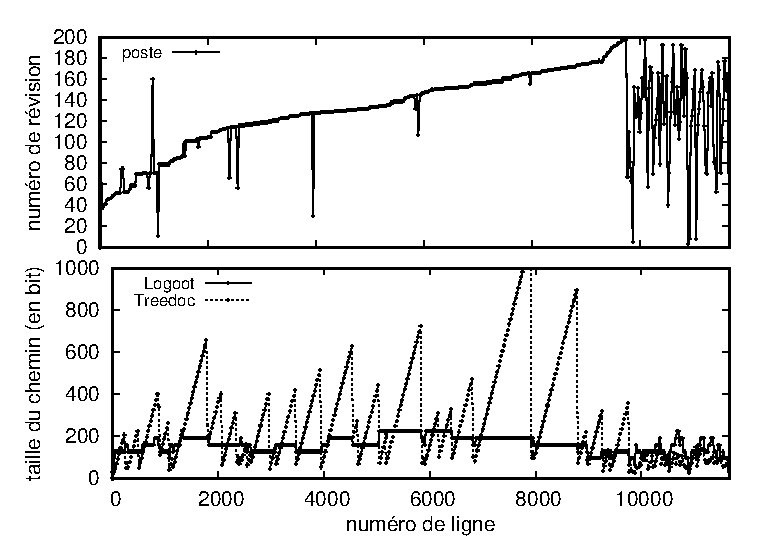
\includegraphics[width=0.8\textwidth]{img/lseq/motivationposte.eps}}
  \hspace{10pt}
  \subfloat[Document Wikipédia principalement édité au début.]
  [\label{repl:img:motivationsB}Document Wikipédia de petite taille
  principalement édité au début.]
  {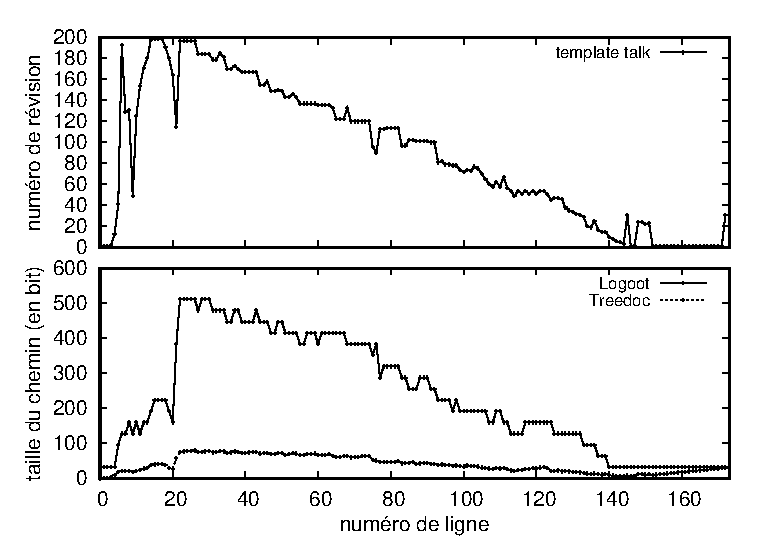
\includegraphics[width=0.8\textwidth]{img/lseq/motivationtemplatetalk.eps}}
  \caption{\label{repl:img:motivations} Taille du chemin alloué pour chaque
    ligne du document. L'axe des abcisses montre le numéro de la ligne
    concernée. L'axe des ordonnées de la partie haute de la figure montre l'âge
    de la ligne. L'axe des ordonnées de la partie basse de la figure montre la
    taille binaire du chemin alloué.}
\end{figure*}

L'encyclopédie Wikipédia répertorie des millions d'articles écrits
collaborativement par sa communauté. Un utilisateur, enregistré ou non, peut
lire un article, et s'il le souhaite, en modifier le contenu. Lorsque ses
modifications sont achevées, il les soumet à Wikipédia. Deux issues possibles :
\begin{inparaenum}[(i)]
\item La contribution est acceptée et sera visible de tous ou
\item la contribution est rejetée car un autre utilisateur a effectué une
  modification en concurrence et l'a soumise en premier. Il faut alors réviser
  la version rejetée afin de l'adapter à la version la plus à jour avant de
  resoumettre si nécessaire.
\end{inparaenum}
Wikipédia garde l'historique des modifications apportées à tous les articles
depuis leur création. Nous sommes alors à même de rejouer les éditions --
nommées révision -- dans l'ordre où elles ont été effectuées. Toutefois, la
concurrence qui pourrait exister dans une édition en temps réelle est effacée
par le processus d'édition même. D'autre part, la granularité est fixée à la
ligne. En cela, les simulations sur corpus Wikipédia diffèrent légèrement de la
réalité.

\begin{itemize}
\item [\textbf{Objectif :}] Montrer que ni Logoot ni Treedoc ne parviennent à
  fournir des identifiants dont la taille soit satisfaisante quel que soit le
  document.
\item [\textbf{Description :}] Logoot est configuré avec une base
  $2^{32}$. Treedoc est configuré pour utiliser sa méthode originelle -- son
  autre heuristique revenant plus ou moins à la stratégie de Logoot. Les
  documents considérés sont des articles extrait de Wikipédia joués sur 200
  révisions. L'un des articles possède à la fin plus de 10k lignes
  principalement ajoutées en fin
  d'article\footnote{\url{https://fr.wikipedia.org/wiki/Liste_des_bureaux_de_poste_français_classés_par_oblitération_Petits_Chiffres}}. L'autre
  article possède seulement 200 lignes mais est principalement édité en
  tête\footnote{\url{https://en.wikipedia.org/wiki/Template_talk:Did_you_know}}.
\item [\textbf{Résultat :}] Les figures~\ref{repl:img:motivationsA}
  et~\ref{repl:img:motivationsB} montrent la taille de l'identifiant associé à
  chaque ligne. Nous observons que Treedoc possède des chemins qui augmentent
  très vite quel que soit le type d'édition. Lorsque le nombre d'insertions
  successives est très grand (cf. figure~\ref{repl:img:motivationsA}) les
  chemins atteignent des tailles prohibitives. Dans ce cas, Logoot se comporte
  mieux. En revanche, dans le cadre de l'édition en tête, Logoot alloue des
  chemins de taille dramatiquement haute et en perpétuelle hausse.
\item [\textbf{Explication :}] Dans les deux types d'édition, Treedoc et Logoot
  allouent des identifiants dont la compléxité est linéaire. Ainsi, plus les
  insertions se succèdent, plus l'arbre est déséquilibré, plus la taille du
  chemin augmente. Mais comme la granularité des chemins Treedoc est binaire
  ($\mathcal{P}\in \mathbb{N}_{<2}.\mathbb{N}_{<2}\ldots\mathbb{N}_{<2}$), cela
  lui permet de conserver des chemins plus petits que ceux de Logoot dans le
  cadre du document édité en tête. D'un autre coté, Logoot a conçu sa stratégie
  pour l'édition en fin. Dès lors, si le comportement suit cette hypothèse, les
  identifiants grossissent par palliers, linéairement certes, mais lentement. En
  revanche, lorsque le comportement d'édition ne coopère pas, les identifiants
  grimpent très rapidement -- comme cela serait le cas avec la seconde
  heuristique de Treedoc.
\end{itemize}

%% Conclusion
Le problème est donc de créer une stratégie d'allocation d'identifiants qui soit
sous-linéaire par rapport au nombre d'insertions dans le document, quel que soit
le comportement d'édition, sachant que ni le nombre ni la position des
insertions ne sont connus par avance. \TODO{Moar.}

%%% Local Variables:
%%% mode: latex
%%% TeX-master: "../../paper"
%%% End:



\chapter{LSeq : une fonction d'allocation sous-linéaire}
\label{repl:chap:lseq}
\minitoc

\lettrine{L}Seq est une fonction d'allocation d'identifiants de taille variable
pour les structures de données sans résolution de conflits dédiées aux
séquences. \LSEQ est composée de trois éléments sous-jacent dont les
comportements, pris individuellement, n'arrivent pas à pourvoir des identifiants
de taille satisfaisante. En revanche, utilisés simultanément, les défaillances
des uns sont comblés par les avantages de autres. En résulte une allocation
d'identifiants polylogarithmique comparé à la taille du document.



\section{Arbre exponentiel}
\label{repl:sec:exponentialtree}

Un arbre exponentiel est une structure d'arbre dont chacun des nœuds possède une
arité maximale $k$ fois supérieure à celle de son parent. Ainsi, si $k$ est fixé
à 2 et que la racine peut accueillir 8 fils, alors chacun de ces fils peut
accueillir à son tour 16 fils etc. Ainsi, la progression du nombre de fils dans
une branche est exponentielle.

\TODO{Moar.}

\begin{figure}
  \centering
  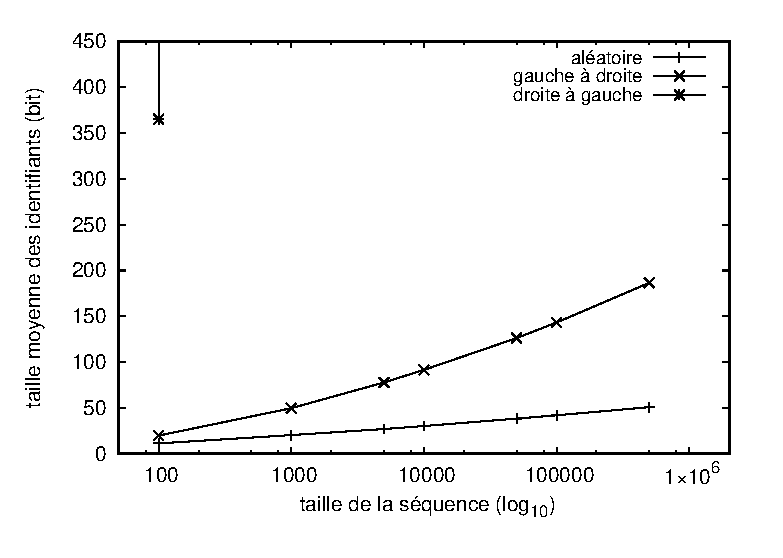
\includegraphics[width=0.8\textwidth]{img/lseq/double.eps}
  \caption{\label{repl:img:exponentialtree} Arbre exponentiel avec stratégie
    d'allocation adaptée à l'édition en fin. L'axe des abscisses montre la
    taille du document sur une échelle logarithmique en base décimale. L'axe des
    ordonnées montre la moyenne des tailles des chemins alloués.}
\end{figure}

\begin{itemize}
\item [\textbf{Objectif :}] Montrer que le chemin des identifiants alloués
  progresse de manière sous-linéaire par rapport à la taille du
  document. Montrer que lorsque le comportement d'édition va à l'opposé de celui
  prévu, l'allocation devient désastreuse.
\item [\textbf{Description :}] Des documents sont créés artificiellement par
  insertions successives de caractères. Trois types de comportement d'édition
  sont simulés :
  \begin{inparaenum}[(i)]
  \item à des positions aléatoire dans le document,
  \item à la fin,
  \item en tête.
  \end{inparaenum}
  La moyenne de la taille des identifiants est mesurée à 100, 1k, 5k, 10k, 50k,
  100k, 500k insertions. La structure utilisée est celle d'un arbre exponentiel
  dont l'arité maximale de départ est fixée à $2^5$.
\item [\textbf{Résultat :}] La figure~\ref{repl:img:exponentialtree} montre les
  résultats des mesures effectuées pendant la simulation. Nous observons que
  lors de l'édition en position aléatoire, l'allocation se comporte extrêmement
  bien avec des chemins de taille logarithmique. Lors de l'édition en fin, la
  taille moyenne des chemins suit une augmentation sous-linéaire par rapport au
  nombre d'insertions dans le document. Finalement, l'édition en tête entraine
  une très forte augmentation de la taille des identifiants.
\item [\textbf{Explication :}] L'édition aléatoire place les éléments au hazard
  dans la séquence. L'arbre est équilibré car nulle branche n'est remplie en
  particulier. À terme, toutes les branches les plus basses sont remplies. Dans
  ce cas, les chemins sont de taille moyenne logarithmiques ce qui constitue la
  borne minimale. Lors de l'édition en queue, les chemins les plus à gauche sont
  alloués réservant de l'espace aux insertions futures. De plus, puisque l'arité
  de l'arbre double à chaque niveau, il peut accueillir deux fois plus de
  chemins à un prix minime (+1 bit/niveau). Pour cette même raison, l'allocation
  est désastreuse lors de l'édition en tête : Quelques insertions suffisent à
  faire augmenter la profondeur de l'arbre. L'arité maximale augmente alors
  rapidement et le prix des identifiants explose.
\end{itemize}


%%% Local Variables:
%%% mode: latex
%%% TeX-master: "../../paper"
%%% End:



\section{Sous-fonctions d'allocation}
\label{repl:sec:suballocation}

Une fonction d'allocation optimale nécessite la connaissance du nombre et de la
position des éditions successives. La fonction peut alors allouer des
identifiants dont la taille est logarithmique comparé à celle du
document. Malheureusement, aucune de ces deux informations n'est disponible dans
l'édition collaborative en temps réel. Dans ces conditions, nous supposerons que
le comportement d'édition est une suite d'éditions adjacentes les unes des
autres -- comme l'édition en tête ou l'édition en fin -- ou à des positions
aléatoires, ou enfin, une composition de ceux-ci.

Afin de gérer ces types d'édition, employer une fonction d'allocation conçue
pour l'édition en fin ne suffit pas. \TODO{Moar. Maybe merge the choice.}

\begin{figure}
  \centering
  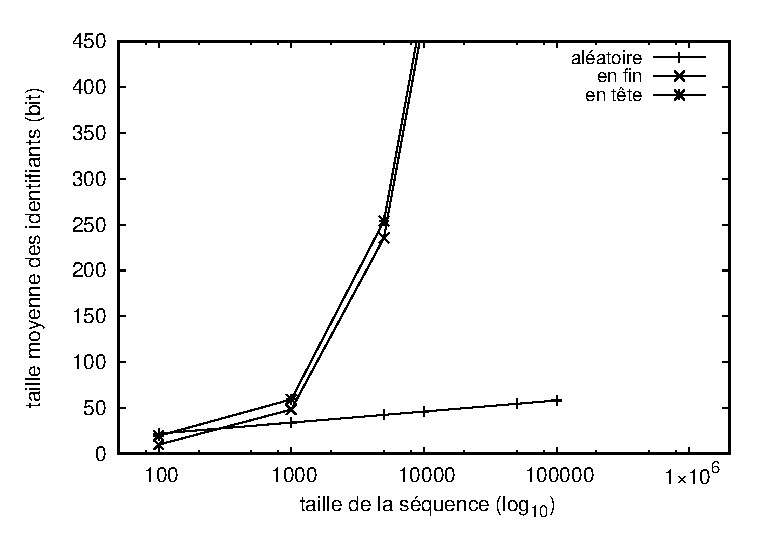
\includegraphics[width=0.8\textwidth]{img/lseq/robin.eps}
  \caption{\label{repl:img:suballocation} Arbre à arité constante et deux
    sous-stratégies d'allocation. L'axe des abscisses montre la taille du
    document sur une échelle logarithmique en base décimale. L'axe des ordonnées
    montre la moyenne des tailles des chemins alloués.}
\end{figure}

\begin{itemize}
\item [\textbf{Objectif :}] Montrer que deux sous-fonctions d'allocation conçues
  avec des objectifs antagonistes mais utilisées ensemble gèrent les
  comportements d'édition triviaux. Montrer que la progression des identifiants
  reste linéaire comparé à la taille du document.
\item [\textbf{Description :}] La simulation concerne trois documents
  grossissant au rythme des opérations d'insertions effectuées respectivement en
  tête, en fin, et aléatoirement. L'arbre a une arité maximale constante. Chaque
  niveau se voit attribuer une sous-fonction d'allocation, i.e., les niveaux
  pairs avec une fonction adaptée à l'édition en tête, et les niveaux impairs
  avec une fonction adaptée à l'édition en fin. Nous mesurons la moyenne des
  chemins composant les identifiants à 100, 1k, 5k, 10k, 50k, 100k insertions.
\item [\textbf{Résultat :}] La figure~\ref{repl:img:suballocation} montre les
  résultats obtenus à la suite de ces simulations. Nous observons tout d'abord
  que les chemins reste logarithmique sous un comportement d'édition
  aléatoire. Nous observons aussi que pour l'édition en tête et l'édition en
  fin, la progression est linéaire mais surtout, quasiment identique dans les
  deux cas.
\item [\textbf{Explication :}] Tout comme pour la
  figure~\ref{repl:img:exponentialtree}, l'édition à des positions aléatoire à
  pour effet d'équilibrer l'arbre représentant le document répliqué. Les chemins
  résultant de ce comportement grandissent de manière logarithmique. Grâce à une
  alternance des sous-fonctions d'allocation, la taille des chemins alloués lors
  de l'édition en tête ou en fin augmente lentement. Malgré tout, la progression
  reste linéaire. De plus, elle augmente deux fois plus rapidement que sans
  cette alternance avec un comportement d'édition favorable. En effet, dans le
  cas de ces simulations, un niveau sur deux composant un chemin est perdu car
  consommé trop vite : la sous-fonction d'allocation assignée à ce niveau
  n'était pas celle conçue pour le comportement d'édition courant.
\end{itemize}



\section{Choix de sous-fonction d'allocation}
\label{repl:sec:allocationchoice}



\section{Algorithmes et complexité}

\TODO{Introduction}

\subsection{Lien arbre -- séquence}

La structure de données répliquée est un arbre mais l'objet manipulé par
l'utilisateur est une séquence. Il est donc nécessaire de fournir les
fonctionnalités d'accès élémentaires afin de faire le lien entre l'arbre et la
séquence.
\begin{inparaenum}[(i)]
\item La fonction \textsc{get} permet d'obtenir l'identifiant à une position
  donnée dans la séquence (cf. §\ref{repl:subsec:get}).
\item La fonction \textsc{indexOf} permet d'obtenir la position d'un
  identifiant (cf. §\ref{repl:subsec:indexof}).
\end{inparaenum}

\subsubsection{get}
\label{repl:subsec:get}

\begin{wrapfigure}{r}{0.6\textwidth}
  \vspace{-35pt} %% (ugly)
  \begin{minipage}[t]{0.6\textwidth}
    \begin{algorithm}[H]
      
\footnotesize
\algrenewcommand{\algorithmiccomment}[1]{\hskip2em$\rhd$ #1}

\newcommand{\comment}[1]{$\rhd$ #1}

\newcommand{\LINEFOR}[2]{%
  \algorithmicfor\ {#1}\ \algorithmicdo\ {#2} %
}

\newcommand{\LINEIFTHEN}[2]{%
  \algorithmicif\ {#1}\ \algorithmicthen\ {#2} %
}

\newcommand{\INDSTATE}[1][1]{\State\hspace{\algorithmicindent}}

\begin{algorithmic}[1]
  \Function{leftmostBranch}{$t \in \mathcal{T}$}{$\, \rightarrow \mathcal{I}$}
  \State \textbf{let} $\langle \_,\, path,\, \_\, children \rangle \leftarrow t$;
  \If {$(|children|=0)$}
  \State \Return t
  \Else
  \State \Return []
  \EndIf
  \EndFunction

  \Function{sumFromLeft}{$t \in \mathcal{T}$, $index \in \mathbb{N}$, $id \in \mathcal{I}$}{$\, \rightarrow \mathcal{I}$}
  \If{$(index = 0)$}
  \State \Return $[id\, |\, \textsc{leftmostBranch}(t)]$;
  \Else
  \State \textbf{let} $i \leftarrow 0$;
  \State \textbf{let} $\langle \_,\, \_,\, children \rangle \leftarrow t$;
  \State \textbf{let} $\langle elem,\, count,\, \_ \leftarrow children[i]$;
  \While {$(index+children)$}
  \State meow
  \EndWhile
  \EndIf
  \EndFunction

  \Statex

  \Function{get}{$index \in \mathbb{N}$}{$\, \rightarrow \mathcal{I}$}
  \State fefef
  \EndFunction

\end{algorithmic}

      \caption{\label{repl:algo:get} Get.}
    \end{algorithm}
  \end{minipage}
  \vspace{-15pt}
\end{wrapfigure}

L'algorithme~\ref{repl:algo:get} présente les instructions de la fonction
\textsc{get} permettant d'obtenir l'identifiant présent à une position donnée
dans la séquence. Celle-ci est nécéssaire lorsque un élément est localement
inséré ou supprimé. En particulier, elle permet de retrouver les identifiants
des éléments adjacents à la position d'insertion. Ces derniers seront ensuite
utilisés afin d'allouer un nouvel identifiant unique.

Afin de retrouver l'identifiant à la position $index$ de la séquence, l'arbre
est parcouru en largeur (cf. ligne~\ref{repl:line:lefttoright}) fixé
arbitrairement de gauche à droite.  Puisque chacun des noeuds sauvegarde le
nombre total de fils qu'il possède, il n'est pas nécessaire de parcourir
l'ensemble des feuilles de l'arbre précedant la position recherchée. Toutefois,
selon la fonction de parcours utilisée pour retrouver la position et la séquence
d'édition ayant rempli la structure, les performances peuvent varier.

\begin{figure}
  \centering
  \begin{tikzpicture}[scale=1.2]
  \newcommand\X{30pt}
  \newcommand\Y{45pt}

  \small
  \draw[dashed, thick] (0pt,0pt) -- node[anchor=south east]{0} (-3.5*\X,-1*\Y);
  \draw[thick, color=darkblue] (0pt,0pt) --
  node[anchor=west]{\DARKBLUE{1}} (-2.5*\X,-1*\Y);
  \draw[thick] (-2.5*\X,-1*\Y) -- node[anchor=east]{3} (-1.5*\X,-2*\Y);
  \draw[thick] (-2.5*\X,-1*\Y) -- node[anchor=east]{7} (-0.5*\X, -2*\Y);
  \draw[thick] (-2.5*\X,-1*\Y) -- node[anchor=west]{11} (0.5*\X,-2*\Y);
  \draw[thick, color=darkblue](0pt,0pt) -- 
  node[anchor=west]{\DARKBLUE{5}} ( 1.5*\X,-1*\Y);
  \draw[thick, color=darkblue] (1.5*\X,-1*\Y) -- 
  node[anchor=west]{\DARKBLUE{4}} (2.5*\X,-2*\Y);
  \draw[dashed, thick] (0pt,0pt) -- node[anchor=south west]{8} ( 3.5*\X,-1*\Y);

  \draw[->, color=darkblue] (-2.5*\X,-1*\Y) -- (-2.5*\X,-10-1*\Y);
  \draw[->] (-1.5*\X,-2*\Y) -- (-1.5*\X,-10-2*\Y);
  \draw[->] (-0.5*\X,-2*\Y) -- (-0.5*\X,-10-2*\Y);
  \draw[->] ( 0.5*\X,-2*\Y) -- ( 0.5*\X,-10-2*\Y);
  \draw[->, color=darkblue] ( 1.5*\X,-1*\Y) -- ( 1.5*\X,-10-1*\Y);
  \draw[->, color=darkblue] ( 2.5*\X,-2*\Y) -- ( 2.5*\X,-10-2*\Y);

  \draw[fill=white, draw=darkblue](-2.5*\X,-14-1*\Y)
  node{\DARKBLUE{\textbf{Q}}}+(-4pt,-4pt)rectangle+(4pt,4pt);
  \draw[fill=white](-1.5*\X,-14-2*\Y)node{\textbf{W}}+(-4pt,-4pt)rectangle+(4pt,4pt);
  \draw[fill=white](-0.5*\X,-14-2*\Y)node{\textbf{E}}+(-4pt,-4pt)rectangle+(4pt,4pt);
  \draw[fill=white]( 0.5*\X,-14-2*\Y)node{\textbf{R}}+(-4pt,-4pt)rectangle+(4pt,4pt);
  \draw[fill=white, draw=darkblue]( 1.5*\X,-14-1*\Y)
  node{\DARKBLUE{\textbf{T}}}+(-4pt,-4pt)rectangle+(4pt,4pt);
  \draw[fill=white, draw=darkblue]( 2.5*\X,-14-2*\Y)
  node{\DARKBLUE{\textbf{Y}}}+(-4pt,-4pt)rectangle+(4pt,4pt);

  \draw[fill=darkblue] (  0pt,  0pt) circle (1pt);
  \draw[fill=black] (-3.5*\X,-1*\Y) circle (1pt);
  \draw[fill=white, draw=darkblue] (-2.5*\X,-1*\Y) circle (1pt);
  \draw[fill=white] (-1.5*\X,-2*\Y) circle (1pt);
  \draw[fill=white] (-0.5*\X,-2*\Y) circle (1pt);
  \draw[fill=white] ( 0.5*\X,-2*\Y) circle (1pt);
  \draw[fill=white, draw=darkblue] ( 1.5*\X,-1*\Y) circle (1pt);
  \draw[fill=white, draw=darkblue] ( 2.5*\X,-2*\Y) circle (1pt);
  \draw[fill=black] ( 3.5*\X,-1*\Y) circle (1pt);

  \draw[->, very thick, densely dashdotted] (15-2.5*\X,-1*\Y) --
  node[anchor=south]{\textbf{search}} (-20+1.5*\X, -1*\Y) -- (-20+2.5*\X, -2*\Y);


\end{tikzpicture}
  \caption{\label{repl:fig:getexample} Exemple de parcours effectué lors de la
    recherche de l'identifiant en position 5 correspondant au caractère 'Y'.}
\end{figure}

La figure~\ref{repl:fig:getexample} montre un exemple de recherche d'identifiant
dans un arbre représentant la séquence 'QWERTY'. La recherche concerne la
position $5$ correspondant au caractère 'Y'. L'arbre est parcouru en partant du
fils gauche de la racine. Ce fils sait que ses sous-branches contiennent 3
caractères. L'algorithme en déduit que le prochain fils de la racine est à la
position 4. En examinant ce second fils, l'algorithme déduit que l'identifiant
recherché est inclue dans l'un de ses fils. Ainsi, il continue l'exploration
dans ce sous-arbre. Lorsqu'il examine le noeud contenant 'Y', il sait que
celui-ci est en position $5$. Par conséquent, il retourne le chemin qu'il a
empreinté pour y parvenir, à savoir [5.4]. Nous pouvons observer dans cet
exemple que si la recherche était parti de la droite, elle n'aurait eu à
parcourir qu'un seul élément intermédiaire (contenant le caractère 'T'), et
aurait donc été plus efficace.


\begin{wraptable}{r}{0.5\textwidth}
  \begin{tabularx}{0.455\textwidth}{@{}Xc@{}}
  \toprule
  \textsc{Editing behavior} & \textsc{Time} \\
  & \ \ \ \ \ \ \ \ \ \textsc{get} \ \ \ \ \ \ \ \ \ \\ \midrule
  Random editing & $\mathcal{O}(2^{\sqrt{\log I}})$ \\
  Monotonic editing & $\mathcal{O}(I)$ \\
  Worst case & $\mathcal{O}(I)$ \\ \bottomrule
\end{tabularx}
  \caption{\label{repl:table:get} Borne supérieure de la complexité temporelle de la fonction \textsc{get} où $I$ est la taille du document.}  
\end{wraptable}

La complexité temporelle de cet algorithme dépend de la séquence d'édition ayant
permit de remplir l'arbre. Ainsi, lorsque l'arbre est rempli aléatoirement, sa
profondeur est faible et un grand nombre d'éléments peuvent être passés. En
revanche, lorsque le comportement d'édition ayant rempli l'arbre est monotone,
une branche de l'arbre seulement est fortement remplie. L'algorithme doit la
parcourir afin de trouver l'identifiant à la position désirée. La complexité est
alors linéaire et correspond au pire cas. Cela s'avère problématique puisque
celle-ci est appelée deux fois par insertion locale. Heureusement, lorsque le
comportement d'édition est monotone, il est facile de se souvenir des bornes
d'insertion : l'une ne change jamais, et l'autre correspond à l'identifiant
nouvellement inséré. Si le comportement d'édition change, l'arbre commence à se
rééquilibrer et les performances se rapprochent de celles de l'édition
aléatoire.


\subsubsection{indexOf}
\label{repl:subsec:indexof}

\begin{wrapfigure}{r}{0.6\textwidth}
  \vspace{-35pt} %% (ugly)
  \begin{minipage}[t]{0.6\textwidth}
    \begin{algorithm}[H]
      
\footnotesize
\algrenewcommand{\algorithmiccomment}[1]{\hskip2em$\rhd$ #1}

\newcommand{\comment}[1]{$\rhd$ #1}

\newcommand{\LINEFOR}[2]{%
  \algorithmicfor\ {#1}\ \algorithmicdo\ {#2} %
}

\newcommand{\LINEIFTHEN}[2]{%
  \algorithmicif\ {#1}\ \algorithmicthen\ {#2} %
}

\newcommand{\INDSTATE}[1][1]{\State\hspace{\algorithmicindent}}

\begin{algorithmic}[1]
  \Function{getIndexesOf}{$t \in \mathcal{T}$, $i \in \mathcal{I}$}{$\, \rightarrow \mathbb{N}^+$}
  \State \textbf{let} $[hd\, |\, tl] \leftarrow i$;
  \State \textbf{let} $\langle \_,\, \_,\, children \rangle \leftarrow t$;
  \State \textbf{let} $index \leftarrow \DARKBLUE{\textsc{binaryIndexOf}}(children,\, hd)$;
  \If{$(index < 0 \wedge |tl| > 0)$}
  \State \Return $[index\, |\, \textsc{getIndexOf}(children[index],\,tl)]$;
  \Else
  \State \Return $[index]$;
  \EndIf
  \EndFunction

  \Statex

  \Function{getSum}{$t \in \mathcal{T}$, $indexes \in \mathbb{N}^+$}{$\, \rightarrow \mathbb{N}$}
  \State \textbf{let} $[hd\, |\, tl] \leftarrow indexes$;
  \State \textbf{let} $\langle \_,\, \_,\, children \rangle \leftarrow t$;
  \State \textbf{let} $sum \leftarrow 0$;
  \State \LINEIFTHEN{$(|tl|>0)$}{$sum \leftarrow \textsc{getSum}(children[hd],\,tl)$;}
  \For{\DARKBLUE{$i$ \textbf{from} 0 \textbf{to} $(hd-1)$}}\label{repl:line:optimization}
  \State \textbf{let} $\langle elem,\,count,\,\_ \rangle \leftarrow children[i]$;
  \State \LINEIFTHEN{$(elem)$}{$sum = sum + 1$;}
  \State $sum = sum + count$;
  \EndFor
  \State \Return $sum$;
  \EndFunction

  \Statex

  \Function{\DARKBLUE{getIndex}}{\DARKBLUE{$t \in \mathcal{T}$, $i \in \mathcal{I}$}}{\DARKBLUE{$\, \rightarrow \mathbb{N}$}}
  \State \textbf{let} $indexes \leftarrow \textsc{getIndexesOf}(t,\,i)$;
  \State \LINEIFTHEN{$(indexes[indexes-1]<0)$}{\Return $-1$;}
  \State \textbf{let} $\langle elem,\, \_,\,\_ \rangle \leftarrow t$;
  \State \textbf{let} $index \leftarrow \textsc{getSum}(t,\,indexes)$;
  \State \LINEIFTHEN{$(elem)$}{$index = index + 1$;}
  \State \Return $index$;
  \EndFunction
\end{algorithmic}

      \caption{\label{repl:algo:indexof} indexOf.}
    \end{algorithm}
  \end{minipage}
  \vspace{-15pt}
\end{wrapfigure}

L'algorithme~\ref{repl:algo:indexof} présente les instructions de la fonction
\textsc{indexOf}. Celle-ci sert essentiellement à placer les éléments réçus dans
la séquence perçue par l'utilisateur.  Celle-ci est divisée en trois :
\begin{inparaenum}[(i)]
\item La fonction \textsc{getIndexesOf} retourne les indices successifs dans les
  listes triées constituants les fils des nœuds de l'arbre. Celle-ci utilise la
  fonction \textsc{binaryIndexOf} possédant un compléxité temporelle
  logarithmique comparée à la taille du tableau trié parcouru.
\item La fonction \textsc{getSum} parcours l'arbre afin d'en déduire l'indice de
  séquence correspondant. Afin de ne pas avoir à parcourir l'entièreté des
  branches, les noeuds sauvegardent le nombre de sous-branches qu'ils possèdent
  (similairement à l'algorithme~\ref{repl:algo:get}).  La
  ligne~\ref{repl:line:optimization} définit la façon dont l'arbre est
  parcouru. Un optimisation consiste à parcourir l'arbre à partir de la borne la
  plus proche de l'indice à la profondeur concernée.
\item La fonction \textsc{indexOf} est composée des deux fonctions
  susmentionnées.
\end{inparaenum}

\TODO{Figure explaining the operation.}

La complexité temporelle de cette fonction est proche de celle de la fonction
\textsc{get} car basée sur le même principe. La seule différence est le surcoût
logarithmique lié à la recherche dichotomique à chaque niveau de l'arbre. Encore
une fois, les complexités linéaires ne sont pas problématiques car ces
opérations peuvent être effectuées en arrière-plan. De plus, l'utilisateur
possède une vue partielle du document. Si les mises à jour ne tombent pas dans
cette fenêtre, la fonction peut arrêter son éxecution.


\subsection{Modification de la structure}

La structure d'arbre représentant le document réparti se modifie au rythme des
insertions et suppressions effectuées par les utilisateurs, qu'ils soient
distants ou non. 

\subsubsection{insert}


\begin{wrapfigure}{r}{0.6\textwidth}
  \vspace{-35pt} %% (ugly)
  \begin{minipage}[t]{0.6\textwidth}
    \begin{algorithm}[H]
      
\footnotesize
\algrenewcommand{\algorithmiccomment}[1]{\hskip2em$\rhd$ #1}

\newcommand{\comment}[1]{$\rhd$ #1}

\newcommand{\LINEFOR}[2]{%
  \algorithmicfor\ {#1}\ \algorithmicdo\ {#2} %
}

\newcommand{\LINEIFTHEN}[2]{%
  \algorithmicif\ {#1}\ \algorithmicthen\ {#2} %
}

\newcommand{\LINEIFTHENELSE}[3]{%
  \algorithmicif\ {#1}\ \algorithmicthen\ {#2} \algorithmicelse\ {#3} %
}

\newcommand{\LET}[2]{%
  \State \textbf{let}\ $#1 \leftarrow #2$%
}

\newcommand{\PIPE}[0]{%
  \,|\,%
}

\newcommand{\INDSTATE}[1][1]{\State\hspace{\algorithmicindent}}

\begin{algorithmic}[1]
  \Function{subInsert}
  {$t \in \mathcal{T},\, indexes \in \mathbb{N}^+,\, i\in\mathcal{I}$}
  {$\, \rightarrow \mathcal{T}$}
  \LET {[index \PIPE indexes]}{indexes};
  \LET {[path \PIPE i]}{i};
  \LET {\langle \_,\, \_,\, count,\, children\rangle}{t};
  \If {$(index<0)$}
  \State \TODO{TODO} 
  \Else
  \EndIf
  \EndFunction

  \Statex

  \Function{insert}
  {$t \in \mathcal{T},\, i \in \mathcal{I}$}
  {$\, \rightarrow \mathcal{T}$}
  \State \Return $\textsc{subInsert}(t,\,\textsc{getIndexesOf}(t,\, i),\,i)$;
  \EndFunction

\end{algorithmic}

      \caption{\label{repl:algo:insert} Insert.}
    \end{algorithm}
  \end{minipage}
  \vspace{-15pt}
\end{wrapfigure}

L'algorithme~\ref{repl:algo:insert} présente les instructions de la fonction
d'insertion.


\subsubsection{delete}


\section{Validation}
\label{repl:sec:validation}

\LSEQ est une fonction d'allocation d'identifiants pour les structures de
données sans resolution de conflits conçue pour les séquences.  Cette section a
deux objectifs. Tout d'abord, elle examine la contribution de chacun des
composants internes à \LSEQ décrits en §\ref{repl:sec:proposal}.  Ensuite, elle
valide expérimentalement les analyses en complexité de \LSEQ faites en
§\ref{repl:sec:complexity}. Enfin, elle montre l'influence de la concurrence sur
l'allocation d'identifiants. Dans toutes ces expérimentations, nous sommes plus
interessés par l'allure des résultats que par leurs valeurs absolues.

\subsection{Référence}

\begin{figure}
  \begin{center}
    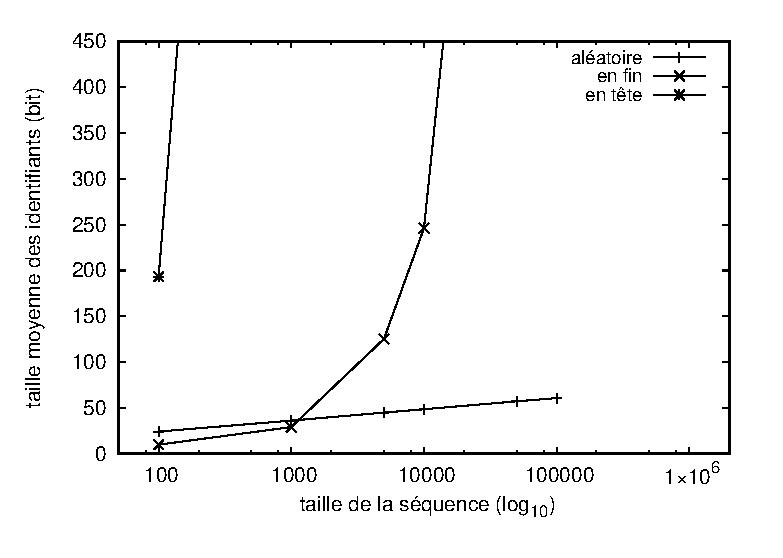
\includegraphics[width=0.8\textwidth]{img/lseq/logoot.eps}
    \caption{\label{repl:img:logoot} Arbre à arité constante avec stratégie
      d'allocation adaptée à l'édition en fin. L'axe des abscisses montre la
      taille du document sur une échelle logarithmique en base décimale. L'axe
      des ordonnées montre la moyenne des tailles des chemins alloués.}
  \end{center}
\end{figure}


\paragraph{Objectif :} Fournir une référence aux futures expérimentations afin
de montrer les améliorations et les dégradations de chaque composant.

\paragraph{Description :} La simulation concerne trois documents artificiels
remplis respectivement par un comportement d'édition aléatoire, un comportement
d'édition monotone de gauche à droite, et un comportement d'édition monotone de
droite à gauche. La fonction d'allocation utilise un arbre d'arité maximale
constante et une seule sous-fonction d'allocation conçue pour l'édition monotone
de gauche à droite. Cette configuration correspond aux stratégies de l'état de
l'art~\cite{preguica2009commutative, weiss2009logoot}.  La moyenne de la taille
des identifiants est mesurée à 100, 1k, 5k, 10k, 50k, 100k insertions.

\paragraph{Résultat :} La figure~\ref{repl:img:logoot} montre les résultats de
cette expérimentation. Nous observons tout d'abord que la taille des
identifiants croît logarithmiquement dans le cas des éditions faites à des
positions aléatoires. Ensuite, les comportements d'édition monotone conduisent
tout deux à une croissance linéaire. Toutefois, l'édition de gauche à droite
reste bien plus efficace que l'édition de droite à gauche.

\paragraph{Explication :} Le comportement d'édition aléatoire conduit à une
structure d'arbre équilibrée. Les identifiants alloués restent petits. Le
comportement d'édition montone de gauche à droite conduit à une croissance
linéaire mais relativement faible. En effet, la stratégie d'allocation employée
est conçue pour ce comportement : Des branches sont laissées disponibles en vue
des prochaines insertions. La taille des identifiants grandit donc
lentement. Toutefois, comme l'arité maximale de l'arbre reste constante, la
structure ne s'adapte pas à la taille du document, d'où la croissance
linéaire. Dans le cas du comportement d'édition monotone de droite à gauche,
l'augmentation de la taille des identifiants est très forte car la stratégie
employée favorise le comportement d'édition opposé. Ainsi les insertions ont tôt
fait de ne plus avoir d'espace disponible conduisant à la création d'un nouvel
espace, i.e. la profondeur de l'arbre augmente. L'augmentation reste linéaire.

\subsection{Arbre exponentiel}

\begin{figure}
  \begin{center}
    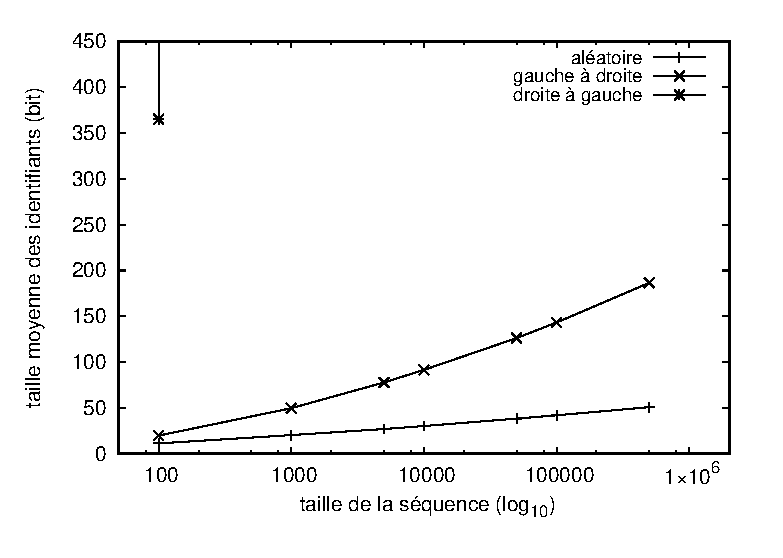
\includegraphics[width=0.8\textwidth]{img/lseq/double.eps}
    \caption{\label{repl:img:exponentialtree} Arbre exponentiel avec stratégie
      d'allocation adaptée à l'édition en fin. L'axe des abscisses montre la
      taille du document sur une échelle logarithmique en base décimale. L'axe
      des ordonnées montre la moyenne des tailles des chemins alloués.}
  \end{center}
\end{figure}

\paragraph{Objectif :} Montrer que l'utilisation d'un arbre exponentiel permet
d'allouer des chemins dont la taille croît de manière polylogarithmique comparé
au nombre d'insertions. Montrer que lorsque le comportement d'édition va à
l'encontre de celui prévu, l'allocation devient désastreuse.

\paragraph{Description :} Trois documents sont créés artificiellement par
insertions successives de caractères. Pour chacun, un comportement d'édition
différent est simulé :
\begin{inparaenum}[(i)]
\item aléatoire,
\item monotone de gauche à droite,
\item montone de droite à gauche.
\end{inparaenum}
La fonction d'allocation est conçue pour l'édition de gauche à droite et utilise
un arbre exponentiel.  La moyenne de la taille des identifiants est mesurée à
100, 1k, 5k, 10k, 50k, 100k, 500k insertions. 

\paragraph{Résultat :} La figure~\ref{repl:img:exponentialtree} montre les
résultats des mesures effectuées pendant la simulation. Nous observons qu'avec
un comportement d'édition aléatoire, et similairement aux mesures de références
(cf. figure~\ref{repl:img:logoot}), la croissance des identifiants est optimale
puisqu'elle suit un logarithme par rapport au nombre d'insertions dans le
document. Lors de l'édition monotone de gauche à droite, la croissance des
chemins est polylogarithmique par rapport au nombre d'insertions. En revanche,
l'édition de droite à gauche entraîne une augmentation quadratique de la taille
des identifiants.

\paragraph{Explication :} L'édition à des positions aléatoires place les
éléments au hazard dans la séquence. L'arbre est équilibré car nulle branche
n'est favorisée. À terme, les branches proches de la racine sont remplies
entièrement. Dans ce cas, les chemins sont de taille logarithmiques ce qui
constitue la borne minimale. Lors du comportement d'édition monotone de gauche à
droite, les chemins les plus à gauche sont alloués réservant de l'espace aux
insertions futures. De plus, puisque l'arité de l'arbre double à chaque niveau,
il peut accueillir deux fois plus de chemins à un prix minime (1 bit additionnel
par niveau). Pour cette même raison, l'allocation est désastreuse lors de
l'édition de droite à gauche : Quelques insertions suffisent à faire augmenter
la profondeur de l'arbre. L'arité maximale augmente alors rapidement et le prix
des identifiants explose. Dans ce cas, la taille des chemins croît de manière
quadratique.


\subsection{Sous-fonctions d'allocation}

\begin{figure}
  \begin{center}
    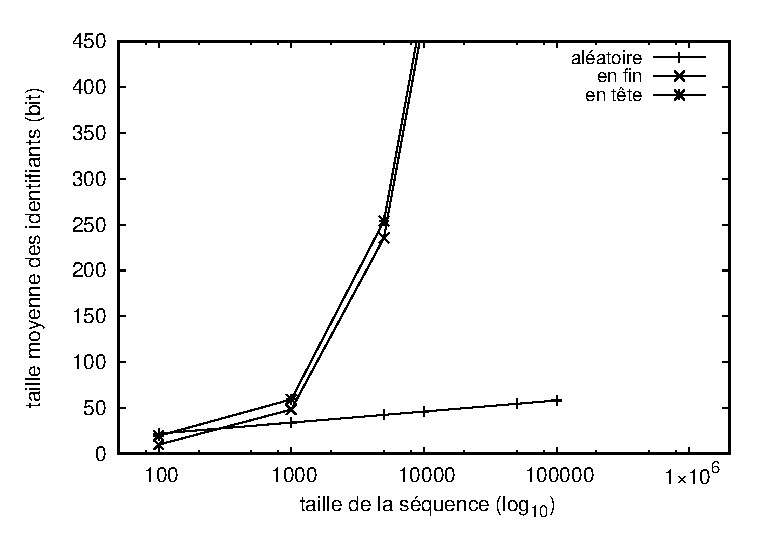
\includegraphics[width=0.8\textwidth]{img/lseq/robin.eps}
    \caption{\label{repl:img:suballocation} Arbre à arité constante et deux
      sous-stratégies d'allocation. L'axe des abscisses montre la taille du
      document sur une échelle logarithmique en base décimale. L'axe des
      ordonnées montre la moyenne des tailles des chemins alloués.}
  \end{center}
\end{figure}

\paragraph{Objectif :} Montrer que deux sous-fonctions d'allocation conçues avec
des objectifs antagonistes mais utilisées ensemble gèrent les comportements
d'édition triviaux. Montrer que la progression des identifiants reste linéaire
comparé à la taille du document.

\paragraph{Description :} La simulation concerne trois documents grossissant au
rythme des opérations d'insertions effectuées respectivement de gauche à droite,
de droite à gauche, et aléatoirement. La fonction d'allocation utilise un arbre
dont l'arité maximale est constante. De plus, chaque niveau se voit attribuer
une sous-fonction d'allocation, i.e., les niveaux pairs avec une fonction conçue
pour l'édition de gauche à droite, et les niveaux impairs avec une fonction
adaptée à l'édition de droite à gauche. Nous mesurons la moyenne des chemins
composant les identifiants à 100, 1k, 5k, 10k, 50k, 100k insertions.

\paragraph{Résultat :} La figure~\ref{repl:img:suballocation} montre les
résultats obtenus à la suite de ces simulations. Nous observons tout d'abord que
les chemins reste logarithmique sous un comportement d'édition aléatoire. Nous
observons aussi que, pour les deux types d'édition monotone, la croissance est
linéaire. De plus, les mesures sont quasiment identiques dans les deux cas.

\paragraph{Explication :} Tout comme pour les expériences précédentes
(cf. figure~\ref{repl:img:logoot} et~\ref{repl:img:exponentialtree}), l'édition
à des positions aléatoires à pour effet d'équilibrer l'arbre représentant le
document répliqué. Les chemins résultant de ce comportement grandissent de
manière logarithmique. Grâce à une alternance des sous-fonctions d'allocation,
la taille des chemins alloués lors des comportements d'édition monotone augmente
lentement. Malgré tout, la progression reste linéaire. De plus, elle augmente
deux fois plus rapidement que sans cette alternance avec un comportement
d'édition favorable (cf. figure~\ref{repl:img:logoot}). En effet, dans le cas de
ces simulations, un niveau sur deux composant un chemin est perdu car consommé
trop vite : La sous-fonction d'allocation assignée à ce niveau n'était pas celle
conçue pour le comportement d'édition courant.


\subsection{Arbre exponentiel et sous-fonctions}

\begin{figure}
  \begin{center}
    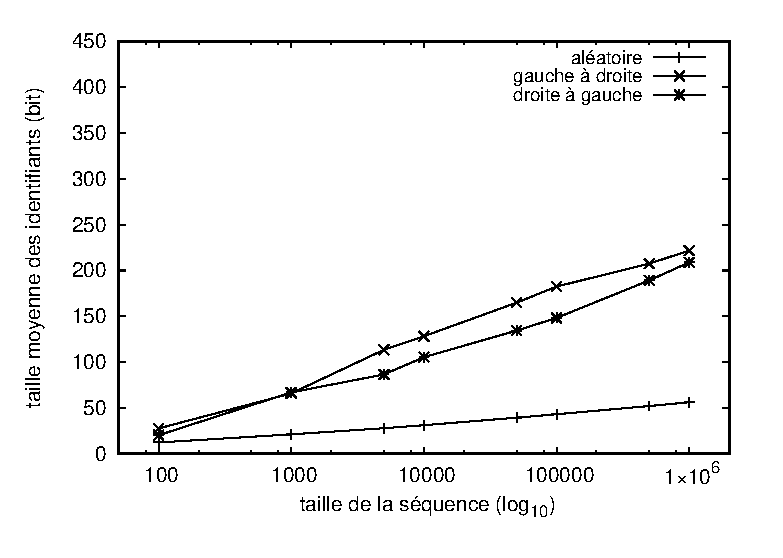
\includegraphics[width=0.8\textwidth]{img/lseq/lseq.eps}
    \caption{\label{repl:img:lseq} Arbre exponentiel avec deux sous-stratégies
      d'allocation. L'axe des abscisses montre la taille du document sur une
      échelle logarithmique en base décimale. L'axe des ordonnées montre la
      moyenne des tailles des chemins alloués.}
  \end{center}
\end{figure}

\paragraph{Objectif :} Montrer que l'utilisation combinée d'un arbre exponentiel
et de sous-fonctions d'allocation permet de pallier les faiblesses respectives
de ceux-ci et d'obtenir une stratégie d'allocation sous-linéaire comparativement
du nombre d'insertions effectuées sur le document. 

\paragraph{Description} Trois documents chacun édité de façon différente :
L'auteur du premier possède un comportement d'édition aléatoire; L'auteur du
second possède un comportement d'édition monotone de gauche à droite; L'auteur
du troisième de droite à gauche. La fonction d'allocation utilise un arbre
exponentiel et deux sous-fonctions d'allocation conçues pour gérer les éditions
monotones. Les sous-fonctions d'allocation sont assignées aléatoirement à chaque
niveau de l'arbre. Les mesures sont faites à 100, 1k, 5k, 10k, 50k, 100k, 500k,
1M insertions.

\paragraph{Résultat :} La figure~\ref{repl:img:lseq} affiche les résultats
obtenus lors de cette expérimentation. Nous observons que la progression de la
taille des identifiants lors du comportement d'édition aléatoire reste
logarithmique. Lors des deux autres comportements d'édition monotone, la
croissance des identifiants suit une progression polylogarithmique comparé au
nombre d'insertions effectuées dans la séquences. Cette observation confirme
l'analyse en complexité spatiale des identifiants
(cf. §\ref{repl:subsec:space}). Cependant, nous observons de petites
différences entre les deux courbes résultant des comportements d'édition monotone.

\paragraph{Explication :} Le comportement d'édition aléatoire conduit à un arbre
exponentiel équilibré, d'où la croissance logarithmique des identifiants. Les
autres cas d'édition sont très similaires car les sous-fonctions d'allocations
ont la même probabilité d'apparaitre. Les différences s'expliquent par les
différents choix lors des exécutions. La progression sous-linéaire s'explique
grâce à l'augmentation d'arité de l'arbre lorsqu'il gagne en profondeur, i.e.,
chaque nœud de l'arbre peut possèder jusqu'à deux fois plus de fils que son
parent ne le peut. Lorsque la sous-fonction d'allocation employée ne s'accorde
pas avec le comportement d'édition, la profondeur de l'arbre est incrémentée
rapidement. Lorsque finalement la bonne sous-fonction d'allocation est trouvée,
celle-ci couvre les dépenses qu'il a fallut déployer pour la trouver, i.e.,
les pertes de niveaux dans l'arbre.

\subsection{Complexité temporelle}

\begin{figure}
  \begin{center}
    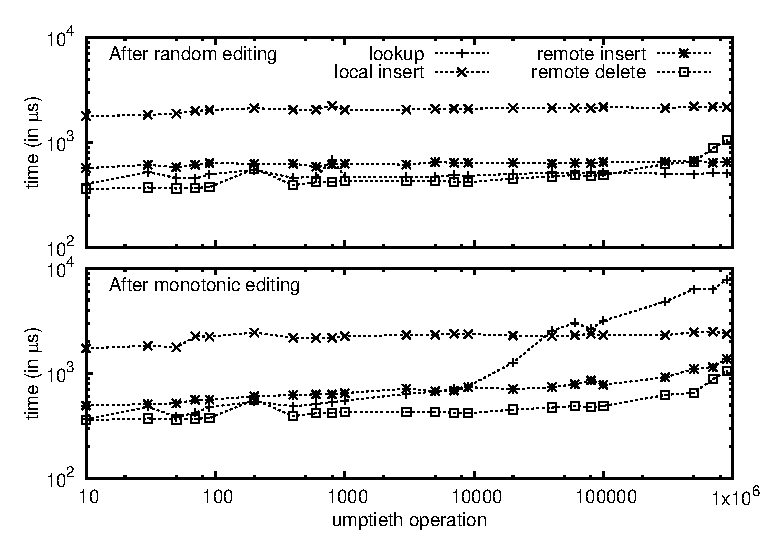
\includegraphics[width=0.8\textwidth]{img/lseq/time.eps}
    \caption{\label{repl:img:time} Performances de la énième opération effectuée
      sur \LSEQ. L'axe des abscisses montre le numéro de la énième
      opération. L'axe des ordonnées montre le temps d'exécution de l'opération
      en microsecondes. La figure du haut considère une structure remplie par
      des insertions aléatoires. La figure du bas considère une structure
      remplies par insertions montones.}
  \end{center}
\end{figure}

\paragraph{Objectif :} Confirmer l'analyse en complexité temporelle de
\LSEQ. Des performances passant à l'echelle sont attendues.

\paragraph{Description :} Cette expérience implique un utilisateur artificiel
unique effectuant des opérations sur sa réplique du document. Le banc d'essai
s'est déroulé sur un \emph{MacBook Pro} comportant un processeur \emph{2.5 GHz
  Intel Core i5}, la version 4.1.1 de \emph{Node.js}, sur une architecture
Darwin 64-bit. Pour chaque opération, un document de $I-1$ caractères est créé
artificiellement. Les mesures s'effectuent sur la $I$\up{ème} opération. Les
opérations prises en compte sont la fonction \textsc{lookup}, la partie locale
de l'insertion, la partie distante de l'insertion, et la partie distante de la
suppression -- la partie locale de cette dernière ne comprend que la propagation
de l'identifiant ciblé aux autres membres. Les mesures sont effectués à
plusieurs reprises sur deux types de documents. Tout d'abord, un document généré
par un comportement d'édition aléatoire, i.e., l'arbre \LSEQ est
équilibré. Ensuite, un document généré par un comportement d'édition monotone,
i.e., une seule branche de l'arbre \LSEQ est remplie. Nous nous intéressons aux
tendences plutôt qu'aux valeurs absolues. En effet, le langage \emph{Javascript}
opère de nombreuses optimisations à la volée. Afin de montrer la contribution
réelle de chacune des opérations, ces optimisations ont été limité au
maximum. Les performances réelles des opérations sont donc nettement meilleures
que celles présentes dans cette expérimentation.

\paragraph{Résultat :} La figure~\ref{repl:img:time} montre les résultats de
cette expérimentation. Nous observons que les valeurs mesurées, dans le cadre
d'un arbre remplies par des éditions aléatoires, ne croissent pratiquement pas,
et ce, quelle que soit l'opération. D'un autre coté, lorsque l'insertion locale
après édition monotone reste stable, nous observons une croissance linéaire du
temps d'exécution de la fonction \textsc{lookup}, et une plus faible évolution
pour les parties distantes des opérations d'insertion et de suppression.

\paragraph{Explication :} Après un comportement d'édition aléatoire, l'arbre de
\LSEQ est équilibré. Par conséquent l'influence d'une opération se limite à un
petit sous ensemble d'éléments composant le document. Par exemple, la fonction
\textsc{lookup} n'a pas besoin d'explorer chaque élément de l'arbre. Elle rejète
rapidement de nombreuses branches sans importances à chaque niveau de l'arbre
car l'indice recherché ne tombe pas dans leur intervalle. Toutefois, cette
remarque n'est pas vraie en ce qui concerne un arbre rempli par un comportement
d'édition monotone. En effet, dans ce cas, la plupart des éléments sont
localisés dans l'une -- et la plus profonde -- des branches de l'arbre. Ainsi,
la fonction \textsc{lookup} va probablement explorer tous les niveaux et
inspecter chaque élément pour en compter le nombre de fils afin d'actualiser son
indice de progression courant. Les mesures concernant les opérations distantes
suivent le même raisonnement. Elles sont plus efficaces car l'exploration des
niveaux utilise la recherche dichotomique.


\subsection{Concurrence}

\begin{figure}
  \begin{center}
    \includegraphics[angle=-90,width=0.8\textwidth]{img/lseq/latency.eps}
    \vspace{25pt}
    \caption{\label{repl:img:latency}Effets de la concurrence sur la taille des
      identifiants. L'axe des abscisses montre le nombre d'opérations effectuées
      sur le document. L'axe des ordonnées montre la taille des messages envoyés
      (en octets).}
  \end{center}
\end{figure}

\paragraph{Objectif :} Montrer que plus la concurrence est élevée, plus les
identifiants alloués sont petits.

\paragraph{Description :} Deux utilisateurs artificiels dont le comportement est
monotone écrivent de gauche à droite un même document. Grâce à
\emph{netem}~\cite{netem}, une latence est ajoutée sur le transport des
messages créant des opérations concurrentes. Les documents atteignent 10k
caractères. Les mesures sur la taille moyenne des messages envoyés sont
effectuées tout au long de l'expérimentation. La fonction d'allocation employée
est celle de \LSEQ : Un arbre exponentiel avec deux sous-fonctions
d'allocations. 

\paragraph{Résultat :} La figure~\ref{repl:img:latency} montre les résultats de
cette expérimentation. Comme attendu, plus la latence est élevée, et donc plus
la concurrence est élevée, plus les messages sont de petite taille. Les
expérimentations sans concurrence présentent donc la borne supérieure des
fonctions d'allocation. La figure~\ref{repl:img:latency} nous montre aussi, avec
une plus fine granularité, la croissance polylogarithmique des messages qui
confirme une seconde fois l'analyse en complexité spatiale des identifiants.

\paragraph{Explication :} Les insertions effectuées par les participants ciblent
une même position dans le document. Toutefois, ils ne prennent connaissance de
cela que quelques temps plus tard, lorsque le message correspondant leur est
parvenu. Ainsi, les opérations sont-elles réellement concurrentes. Les
insertions étant effectuées en concurrence à la même position dans la séquence,
les opérations partagent le même espace d'allocation. Entre autre, les
identifiants ont une chance d'obtenir le même chemin dans l'arbre. En moyenne,
ils sont plus rapproché les uns des autres. Il est important de noter que les
documents résultant de ces expérimentations sont différents. En d'autres termes,
la série de caractères composant le document est différente en fonction de la
latence.


%%% Local Variables:
%%% mode: latex
%%% TeX-master: "../../paper"
%%% End:



\section{Conclusion}
\label{repl:sec:conclusion}

Dans ce chapitre, nous avons présenté \LSEQ, un fonction d'allocation
d'identifiants pour les structures de données sans résolution de conflits
conçues pour les séquences. 

\begin{itemize}
\item [\textbf{QR B.}] \textbf{Afin d'éviter tout protocole additionnel de
    relocalisation des identifiants, comment allouer ces identifiants pour que
    leur taille soit directement sous-linéaire.}
\end{itemize}

L'utilisation d'un arbre exponentiel en tant que structure permet d'améliorer
l'allocation sur des comportements d'édition au prix d'un pire cas plus
honéreux. Ce pire cas est rendu difficile à atteindre grâce à l'utilisation de
deux sous-fonctions d'allocation conçues pour les comportement d'édition
monotone. Si malgré tout un utilisateur malintentionné tente d'obtenir de tels
identifiants, la différence entre les identifiants attendus et les identifiants
incriminés est telle qu'il est facile de confondre le coupable, et de prendre
les mesures correspondantes. La complexité des identifiants \LSEQ est bornée par
un polylogarithme comparativement au nombre d'insertions effectuées sur la
séquence.

Le chapitre~\ref{editor:chap:crate} décrit un éditeur de texte collaboratif
temps réel. Dans ce contexte, chaque identifiant généré doit être envoyé au
reste des participants à la session d'édition. Maintenir une croissance des
identifiants sous-linéaire permet de passer à l'échelle. Par conséquent, la
structure ne nécessite pas de relocalisation d'identifiants s'avérant hors de
prix.



%%% Local Variables:
%%% mode: latex
%%% TeX-master: "../../paper"
%%% End:
